\documentclass[]{report}
\usepackage{lmodern}
\usepackage{amssymb,amsmath}
\usepackage{ifxetex,ifluatex}
\usepackage{fixltx2e} % provides \textsubscript
\ifnum 0\ifxetex 1\fi\ifluatex 1\fi=0 % if pdftex
  \usepackage[T1]{fontenc}
  \usepackage[utf8]{inputenc}
\else % if luatex or xelatex
  \ifxetex
    \usepackage{mathspec}
  \else
    \usepackage{fontspec}
  \fi
  \defaultfontfeatures{Ligatures=TeX,Scale=MatchLowercase}
\fi
% use upquote if available, for straight quotes in verbatim environments
\IfFileExists{upquote.sty}{\usepackage{upquote}}{}
% use microtype if available
\IfFileExists{microtype.sty}{%
\usepackage{microtype}
\UseMicrotypeSet[protrusion]{basicmath} % disable protrusion for tt fonts
}{}
\usepackage[margin=1in]{geometry}
\usepackage{hyperref}
\hypersetup{unicode=true,
            pdftitle={DATA 624 PROJECT 2: Regression modeling - PH prediction},
            pdfauthor={Sang Yoon (Andy) Hwang},
            pdfborder={0 0 0},
            breaklinks=true}
\urlstyle{same}  % don't use monospace font for urls
\usepackage{color}
\usepackage{fancyvrb}
\newcommand{\VerbBar}{|}
\newcommand{\VERB}{\Verb[commandchars=\\\{\}]}
\DefineVerbatimEnvironment{Highlighting}{Verbatim}{commandchars=\\\{\}}
% Add ',fontsize=\small' for more characters per line
\usepackage{framed}
\definecolor{shadecolor}{RGB}{248,248,248}
\newenvironment{Shaded}{\begin{snugshade}}{\end{snugshade}}
\newcommand{\KeywordTok}[1]{\textcolor[rgb]{0.13,0.29,0.53}{\textbf{#1}}}
\newcommand{\DataTypeTok}[1]{\textcolor[rgb]{0.13,0.29,0.53}{#1}}
\newcommand{\DecValTok}[1]{\textcolor[rgb]{0.00,0.00,0.81}{#1}}
\newcommand{\BaseNTok}[1]{\textcolor[rgb]{0.00,0.00,0.81}{#1}}
\newcommand{\FloatTok}[1]{\textcolor[rgb]{0.00,0.00,0.81}{#1}}
\newcommand{\ConstantTok}[1]{\textcolor[rgb]{0.00,0.00,0.00}{#1}}
\newcommand{\CharTok}[1]{\textcolor[rgb]{0.31,0.60,0.02}{#1}}
\newcommand{\SpecialCharTok}[1]{\textcolor[rgb]{0.00,0.00,0.00}{#1}}
\newcommand{\StringTok}[1]{\textcolor[rgb]{0.31,0.60,0.02}{#1}}
\newcommand{\VerbatimStringTok}[1]{\textcolor[rgb]{0.31,0.60,0.02}{#1}}
\newcommand{\SpecialStringTok}[1]{\textcolor[rgb]{0.31,0.60,0.02}{#1}}
\newcommand{\ImportTok}[1]{#1}
\newcommand{\CommentTok}[1]{\textcolor[rgb]{0.56,0.35,0.01}{\textit{#1}}}
\newcommand{\DocumentationTok}[1]{\textcolor[rgb]{0.56,0.35,0.01}{\textbf{\textit{#1}}}}
\newcommand{\AnnotationTok}[1]{\textcolor[rgb]{0.56,0.35,0.01}{\textbf{\textit{#1}}}}
\newcommand{\CommentVarTok}[1]{\textcolor[rgb]{0.56,0.35,0.01}{\textbf{\textit{#1}}}}
\newcommand{\OtherTok}[1]{\textcolor[rgb]{0.56,0.35,0.01}{#1}}
\newcommand{\FunctionTok}[1]{\textcolor[rgb]{0.00,0.00,0.00}{#1}}
\newcommand{\VariableTok}[1]{\textcolor[rgb]{0.00,0.00,0.00}{#1}}
\newcommand{\ControlFlowTok}[1]{\textcolor[rgb]{0.13,0.29,0.53}{\textbf{#1}}}
\newcommand{\OperatorTok}[1]{\textcolor[rgb]{0.81,0.36,0.00}{\textbf{#1}}}
\newcommand{\BuiltInTok}[1]{#1}
\newcommand{\ExtensionTok}[1]{#1}
\newcommand{\PreprocessorTok}[1]{\textcolor[rgb]{0.56,0.35,0.01}{\textit{#1}}}
\newcommand{\AttributeTok}[1]{\textcolor[rgb]{0.77,0.63,0.00}{#1}}
\newcommand{\RegionMarkerTok}[1]{#1}
\newcommand{\InformationTok}[1]{\textcolor[rgb]{0.56,0.35,0.01}{\textbf{\textit{#1}}}}
\newcommand{\WarningTok}[1]{\textcolor[rgb]{0.56,0.35,0.01}{\textbf{\textit{#1}}}}
\newcommand{\AlertTok}[1]{\textcolor[rgb]{0.94,0.16,0.16}{#1}}
\newcommand{\ErrorTok}[1]{\textcolor[rgb]{0.64,0.00,0.00}{\textbf{#1}}}
\newcommand{\NormalTok}[1]{#1}
\usepackage{graphicx,grffile}
\makeatletter
\def\maxwidth{\ifdim\Gin@nat@width>\linewidth\linewidth\else\Gin@nat@width\fi}
\def\maxheight{\ifdim\Gin@nat@height>\textheight\textheight\else\Gin@nat@height\fi}
\makeatother
% Scale images if necessary, so that they will not overflow the page
% margins by default, and it is still possible to overwrite the defaults
% using explicit options in \includegraphics[width, height, ...]{}
\setkeys{Gin}{width=\maxwidth,height=\maxheight,keepaspectratio}
\IfFileExists{parskip.sty}{%
\usepackage{parskip}
}{% else
\setlength{\parindent}{0pt}
\setlength{\parskip}{6pt plus 2pt minus 1pt}
}
\setlength{\emergencystretch}{3em}  % prevent overfull lines
\providecommand{\tightlist}{%
  \setlength{\itemsep}{0pt}\setlength{\parskip}{0pt}}
\setcounter{secnumdepth}{0}

%%% Use protect on footnotes to avoid problems with footnotes in titles
\let\rmarkdownfootnote\footnote%
\def\footnote{\protect\rmarkdownfootnote}

%%% Change title format to be more compact
\usepackage{titling}

% Create subtitle command for use in maketitle
\newcommand{\subtitle}[1]{
  \posttitle{
    \begin{center}\large#1\end{center}
    }
}

\setlength{\droptitle}{-2em}

  \title{DATA 624 PROJECT 2: Regression modeling - PH prediction}
    \pretitle{\vspace{\droptitle}\centering\huge}
  \posttitle{\par}
    \author{Sang Yoon (Andy) Hwang}
    \preauthor{\centering\large\emph}
  \postauthor{\par}
      \predate{\centering\large\emph}
  \postdate{\par}
    \date{10 December 2019}

% set plain style for page numbers
\usepackage[margin=1in]{geometry}
\usepackage{fancyhdr}
\pagestyle{fancy}
\fancyhead[LE,RO]{\textbf{Group 2}}
\fancyhead[RE,LO]{\textbf{Project 2: Predicting PH}}
\raggedbottom
\setlength{\parskip}{1em}

% change font
\usepackage{fontspec}
\setmainfont{Arial}

% format titles 
\usepackage{xcolor}
\usepackage{sectsty}
\usepackage{etoolbox}
\usepackage{titling}
\definecolor{prettyblue}{RGB}{84, 144, 240}
\definecolor{bluegray}{RGB}{98, 107, 115}
\pretitle{\begin{center}\Huge\color{prettyblue}\textbf}
\posttitle{\par\LARGE\color{gray}DATA 624 - Predictive Analytics\linebreak Group 2\end{center}}
\preauthor{\begin{center}\large\textbf{Group Members:}\linebreak\textit}
\postauthor{\end{center}}

% Format chapter output
\usepackage{titlesec}
\titleclass{\part}{top}
\titleclass{\chapter}{straight}
\titleformat{\chapter}
  {\normalfont\color{prettyblue}\LARGE\bfseries}{\thechapter}{1em}{}
\titlespacing*{\chapter}{0pt}{3.5ex plus 1ex minus .2ex}{2.3ex plus .2ex}


% create color block quotes
\usepackage{tcolorbox}
\newtcolorbox{myquote}{colback=purple!05!white, colframe=purple!75!black}
\renewenvironment{quote}{\begin{myquote}}{\end{myquote}}

% kable 
\usepackage{tabu}


% multicolumn
\usepackage{multicol}

% bullets
\newenvironment{tight_enumerate}{
\begin{enumerate}
  \setlength{\itemsep}{0pt}
  \setlength{\parskip}{0pt}
  }{\end{enumerate}}
  
\newenvironment{tight_itemize}{
\begin{itemize}
  \setlength{\topsep}{0pt}
  \setlength{\itemsep}{0pt}
  \setlength{\parskip}{0pt}
  \setlength{\parsep}{0pt}
  }{\end{itemize}}

\usepackage{paralist}

%hyperlink
\usepackage{hyperref}
\hypersetup{
    colorlinks=true,
    linkcolor=bluegray,
    filecolor=magenta,      
    urlcolor=cyan}

\usepackage{graphicx}
\usepackage{wrapfig}
\usepackage{booktabs}
\definecolor{yale}{RGB}{13,77,146}
\usepackage[font={color=yale,bf,scriptsize},figurename=Fig.,belowskip=0pt,aboveskip=0pt]{caption}
\usepackage{floatrow}
\floatsetup[figure]{capposition=above}
\floatsetup[table]{capposition=above}
\setlength{\abovecaptionskip}{1pt}
\setlength{\belowcaptionskip}{1pt}
\setlength{\textfloatsep}{2pt plus 0.5pt minus 0.5pt}
\setlength{\intextsep}{2pt plus 0.5pt minus 0.5pt}
\usepackage{booktabs}
\usepackage{longtable}
\usepackage{array}
\usepackage{multirow}
\usepackage{wrapfig}
\usepackage{float}
\usepackage{colortbl}
\usepackage{pdflscape}
\usepackage{tabu}
\usepackage{threeparttable}
\usepackage{threeparttablex}
\usepackage[normalem]{ulem}
\usepackage{makecell}
\usepackage{xcolor}

\begin{document}
\maketitle

{
\setcounter{tocdepth}{1}
\tableofcontents
}
\thispagestyle{empty} \newpage
\clearpage
\pagenumbering{arabic}

\chapter*{Introduction}\label{intro}
\addcontentsline{toc}{chapter}{Introduction}

The goal of this project is to predict \texttt{PH}, a measure of
acidity/alkalinity, using train data set from a beverage company which
consists of 2571 rows of data and 33 variables. After creating models
based on training data, we will test on scoring set of 267 rows with 32
variables (excluding target variable which is \texttt{PH} in our
training set)

As a group project, each member of the group is responsible for creating
their own models of choice. For instance, my own selections were
\texttt{PLS} and \texttt{Bagged\ Tree}. However, the choice of models
can be altered after careful review of data exploration - it may require
different type of model in case data suffers from outliers or any other
data related issues.

Explaining why some necessary steps were applied before modeling and
model A was preferred to Model B is often a topic in academic papers
which is a meaningful topic that helps audience learn the concept of
bagged regression and least square method better.

The final version of report will contain all of our approaches with
results of \texttt{MAPE} for each model with detailed explanation of
why/what/how each model of choice was constructed.

\chapter{Data Exploration}\label{data-exploration}

\section{Data dictionary}\label{data-dictionary}

The table below describes the variables in the train data set.

\begin{table}[H]

\caption{\label{tab:unnamed-chunk-3}Data dictionary}
\centering
\fontsize{8}{10}\selectfont
\begin{tabular}[t]{llrrll}
\toprule
\textbf{Name} & \textbf{Type} & \textbf{MD code} & \textbf{Length} & \textbf{Measurement Type} & \textbf{Excluded}\\
\midrule
\rowcolor{gray!6}  Test Time & Double & -9999 & 8 & m/d/yy h:mm Am/Pm & Auto\\
Brand Code & Double & -9999 & 8 & General & Categorical\\
\rowcolor{gray!6}  Carb Volume & Double & -9999 & 8 & General & Auto\\
Fill Ounces & Double & -9999 & 8 & General & Auto\\
\rowcolor{gray!6}  PC Volume & Double & -9999 & 8 & General & Auto\\
\addlinespace
Carb Pressure & Double & -9999 & 8 & General & Auto\\
\rowcolor{gray!6}  Carb Temp & Double & -9999 & 8 & General & Auto\\
PSC & Double & -9999 & 8 & General & Auto\\
\rowcolor{gray!6}  PSC Fill & Double & -9999 & 8 & General & Auto\\
PSC CO2 & Double & -9999 & 8 & General & Auto\\
\addlinespace
\rowcolor{gray!6}  Mnf Flow & Double & -9999 & 8 & General & Auto\\
Carb Pressure1 & Double & -9999 & 8 & General & Auto\\
\rowcolor{gray!6}  Fill Pressure & Double & -9999 & 8 & General & Auto\\
Hyd Pressure1 & Double & -9999 & 8 & General & Auto\\
\rowcolor{gray!6}  Hyd Pressure2 & Double & -9999 & 8 & General & Auto\\
\addlinespace
Hyd Pressure3 & Double & -9999 & 8 & General & Auto\\
\rowcolor{gray!6}  Hyd Pressure4 & Double & -9999 & 8 & General & Auto\\
Filler Level & Double & -9999 & 8 & General & Auto\\
\rowcolor{gray!6}  Filler Speed & Double & -9999 & 8 & General & Auto\\
Temperature & Double & -9999 & 8 & General & Auto\\
\addlinespace
\rowcolor{gray!6}  Usage cont & Double & -9999 & 8 & General & Auto\\
Carb Flow & Double & -9999 & 8 & General & Auto\\
\rowcolor{gray!6}  Density & Double & -9999 & 8 & General & Auto\\
MFR & Double & -9999 & 8 & General & Auto\\
\rowcolor{gray!6}  Balling & Double & -9999 & 8 & General & Auto\\
\addlinespace
Pressure Vacuum & Double & -9999 & 8 & General & Auto\\
\rowcolor{gray!6}  PH & Double & -9999 & 8 & General & Auto\\
Oxygen Filler & Double & -9999 & 8 & General & Auto\\
\rowcolor{gray!6}  Bowl Setpoint & Double & -9999 & 8 & General & Auto\\
Pressure Setpoint & Double & -9999 & 8 & General & Auto\\
\addlinespace
\rowcolor{gray!6}  Air Pressurer & Double & -9999 & 8 & General & Auto\\
Alch Rel & Double & -9999 & 8 & General & Auto\\
\rowcolor{gray!6}  Carb Rel & Double & -9999 & 8 & General & Auto\\
Balling Lvl & Double & -9999 & 8 & General & Auto\\
\rowcolor{gray!6}  sample & Double & -999999998 & 8 & General & Auto\\
\bottomrule
\end{tabular}
\end{table}

\section{Summary statistics}\label{summary-statistics}

Since we are implementing models which do not require hard assumptions
of joint distribution of variables, normality assumption is not
required. We will focus on how to handle missing values only.

It is apparent, from below, that we have variables that are missing
values - we will impute NULLs with MICE later on.

\begin{table}[H]

\caption{\label{tab:unnamed-chunk-4}Summary statistics}
\centering
\fontsize{8}{10}\selectfont
\begin{tabular}[t]{lrrrrrrrr}
\toprule
\textbf{metric} & \textbf{missing} & \textbf{min} & \textbf{Q1} & \textbf{mean} & \textbf{median} & \textbf{Q3} & \textbf{max} & \textbf{sd}\\
\midrule
\rowcolor{gray!6}  AirPressurer & 0 & 140.8000000 & 142.2000000 & 142.8339946 & 142.6000000 & 143.000000 & 148.200 & 1.2119170\\
AlchRel & 9 & 5.2800000 & 6.5400000 & 6.8974161 & 6.5600000 & 7.240000 & 8.620 & 0.5052753\\
\rowcolor{gray!6}  Balling & 1 & -0.1700000 & 1.4960000 & 2.1977696 & 1.6480000 & 3.292000 & 4.012 & 0.9310914\\
BallingLvl & 1 & 0.0000000 & 1.3800000 & 2.0500078 & 1.4800000 & 3.140000 & 3.660 & 0.8703089\\
\rowcolor{gray!6}  BowlSetpoint & 2 & 70.0000000 & 100.0000000 & 109.3265862 & 120.0000000 & 120.000000 & 140.000 & 15.3031541\\
\addlinespace
CarbFlow & 2 & 26.0000000 & 1144.0000000 & 2468.3542234 & 3028.0000000 & 3186.000000 & 5104.000 & 1073.6964743\\
\rowcolor{gray!6}  CarbPressure & 27 & 57.0000000 & 65.6000000 & 68.1895755 & 68.2000000 & 70.600000 & 79.400 & 3.5382039\\
CarbPressure1 & 32 & 105.6000000 & 119.0000000 & 122.5863726 & 123.2000000 & 125.400000 & 140.200 & 4.7428819\\
\rowcolor{gray!6}  CarbRel & 10 & 4.9600000 & 5.3400000 & 5.4367825 & 5.4000000 & 5.540000 & 6.060 & 0.1287183\\
CarbTemp & 26 & 128.6000000 & 138.4000000 & 141.0949234 & 140.8000000 & 143.800000 & 154.000 & 4.0373861\\
\addlinespace
\rowcolor{gray!6}  CarbVolume & 10 & 5.0400000 & 5.2933333 & 5.3701978 & 5.3466667 & 5.453333 & 5.700 & 0.1063852\\
Density & 1 & 0.2400000 & 0.9000000 & 1.1736498 & 0.9800000 & 1.620000 & 1.920 & 0.3775269\\
\rowcolor{gray!6}  FillerLevel & 20 & 55.8000000 & 98.3000000 & 109.2523716 & 118.4000000 & 120.000000 & 161.200 & 15.6984241\\
FillerSpeed & 57 & 998.0000000 & 3888.0000000 & 3687.1988862 & 3982.0000000 & 3998.000000 & 4030.000 & 770.8200208\\
\rowcolor{gray!6}  FillOunces & 38 & 23.6333333 & 23.9200000 & 23.9747546 & 23.9733333 & 24.026667 & 24.320 & 0.0875299\\
\addlinespace
FillPressure & 22 & 34.6000000 & 46.0000000 & 47.9221656 & 46.4000000 & 50.000000 & 60.400 & 3.1775457\\
\rowcolor{gray!6}  HydPressure1 & 11 & -0.8000000 & 0.0000000 & 12.4375781 & 11.4000000 & 20.200000 & 58.000 & 12.4332538\\
HydPressure2 & 15 & 0.0000000 & 0.0000000 & 20.9610329 & 28.6000000 & 34.600000 & 59.400 & 16.3863066\\
\rowcolor{gray!6}  HydPressure3 & 15 & -1.2000000 & 0.0000000 & 20.4584507 & 27.6000000 & 33.400000 & 50.000 & 15.9757236\\
HydPressure4 & 30 & 52.0000000 & 86.0000000 & 96.2888627 & 96.0000000 & 102.000000 & 142.000 & 13.1225594\\
\addlinespace
\rowcolor{gray!6}  MFR & 212 & 31.4000000 & 706.3000000 & 704.0492582 & 724.0000000 & 731.000000 & 868.600 & 73.8983094\\
MnfFlow & 2 & -100.2000000 & -100.0000000 & 24.5689373 & 65.2000000 & 140.800000 & 229.400 & 119.4811263\\
\rowcolor{gray!6}  OxygenFiller & 12 & 0.0024000 & 0.0220000 & 0.0468426 & 0.0334000 & 0.060000 & 0.400 & 0.0466436\\
PCVolume & 39 & 0.0793333 & 0.2391667 & 0.2771187 & 0.2713333 & 0.312000 & 0.478 & 0.0606953\\
\rowcolor{gray!6}  PH & 4 & 7.8800000 & 8.4400000 & 8.5456486 & 8.5400000 & 8.680000 & 9.360 & 0.1725162\\
\addlinespace
PressureSetpoint & 12 & 44.0000000 & 46.0000000 & 47.6153966 & 46.0000000 & 50.000000 & 52.000 & 2.0390474\\
\rowcolor{gray!6}  PressureVacuum & 0 & -6.6000000 & -5.6000000 & -5.2161027 & -5.4000000 & -5.000000 & -3.600 & 0.5699933\\
PSC & 33 & 0.0020000 & 0.0480000 & 0.0845737 & 0.0760000 & 0.112000 & 0.270 & 0.0492690\\
\rowcolor{gray!6}  PSCCO2 & 39 & 0.0000000 & 0.0200000 & 0.0564139 & 0.0400000 & 0.080000 & 0.240 & 0.0430387\\
PSCFill & 23 & 0.0000000 & 0.1000000 & 0.1953689 & 0.1800000 & 0.260000 & 0.620 & 0.1177817\\
\addlinespace
\rowcolor{gray!6}  Temperature & 14 & 63.6000000 & 65.2000000 & 65.9675401 & 65.6000000 & 66.400000 & 76.200 & 1.3827783\\
Usagecont & 5 & 12.0800000 & 18.3600000 & 20.9929618 & 21.7900000 & 23.755000 & 25.900 & 2.9779364\\
\bottomrule
\end{tabular}
\end{table}

Since \texttt{Brand\ code} is categorical, creating summary statistics
was not possible. Instead, we implemented table summary of the
distribution of each value. Note that we are missing 120 values.

\begin{table}[H]

\caption{\label{tab:unnamed-chunk-5}Frequency distribution of BrandCode}
\centering
\fontsize{8}{10}\selectfont
\begin{tabular}[t]{lr}
\toprule
\textbf{Var1} & \textbf{Freq}\\
\midrule
\rowcolor{gray!6}  A & 293\\
B & 1239\\
\rowcolor{gray!6}  C & 304\\
D & 615\\
\rowcolor{gray!6}  NA & 120\\
\bottomrule
\end{tabular}
\end{table}

\section{Visualizations}\label{visualizations}

\subsection{Missing data}\label{missing-data}

With the help of visualization, it is easier to navigate how much each
variable is missing. Note that \texttt{MFR} is the most missing
variable.

\begin{center}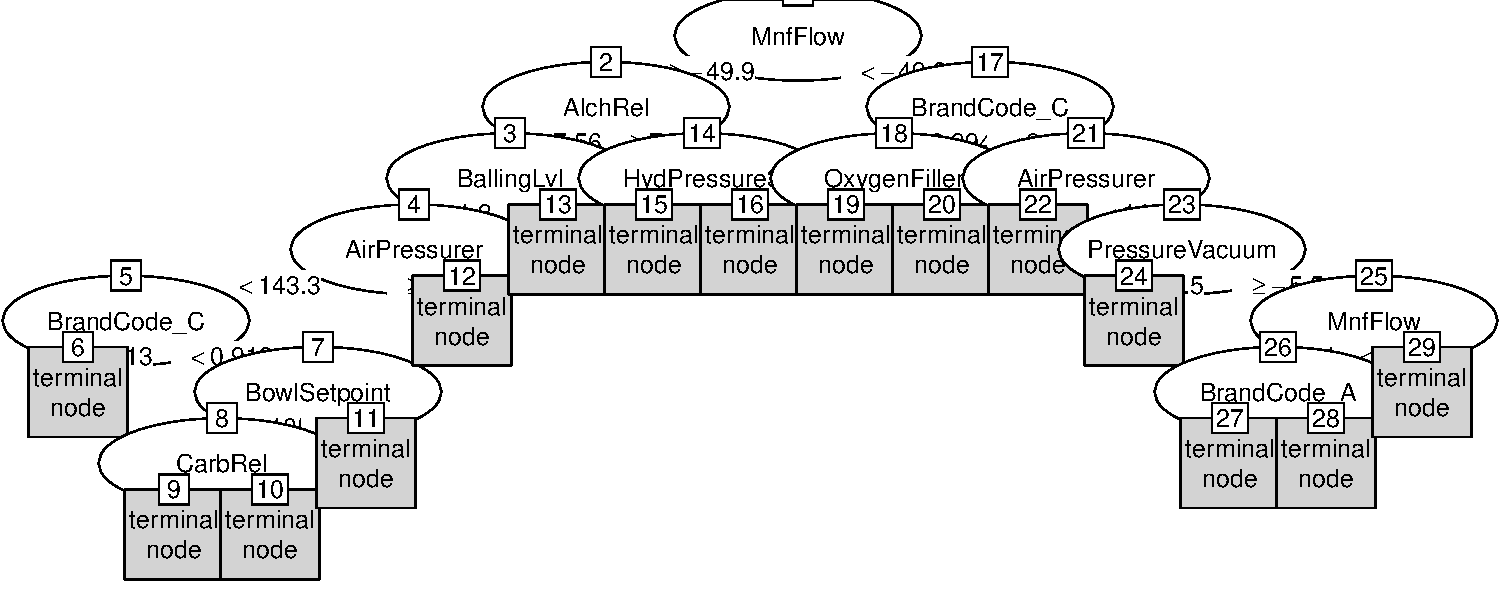
\includegraphics{Proj2-AndyHwang_files/figure-latex/unnamed-chunk-6-1} \end{center}

\subsection{Univariate distributions}\label{univariate-distributions}

We notice that there are some variables such as \texttt{Temperature} and
\texttt{Oxygen\ Filler} that are highly positively skewed. There are
potentials of presence of outliers for skewed variables.

\begin{center}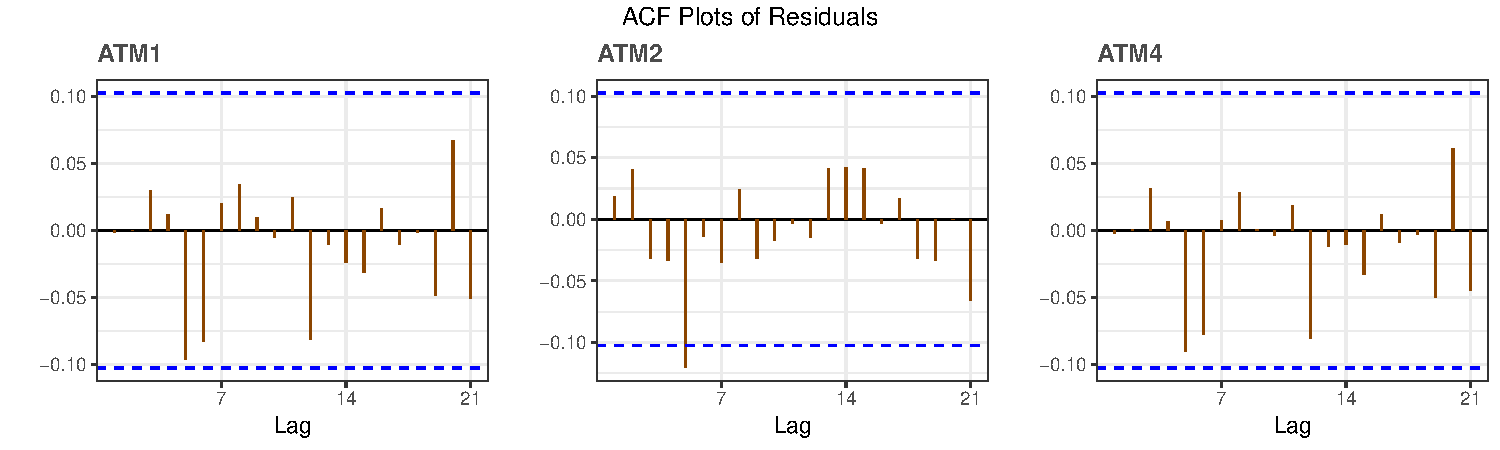
\includegraphics{Proj2-AndyHwang_files/figure-latex/unnamed-chunk-7-1} \end{center}

As we expected, there are many outliers in \texttt{Temperature} and
\texttt{Oxygen\ Filler}. Note that \texttt{MFR} greatly suffers from the
presence of outliers.

From the presence of multiple outliers, we then have to explain
why/what/how we revise our initial model choice of \texttt{Bagged\ Tree}
and apply necessary adjustment before applying \texttt{PLS}.

Ensembled model such as\texttt{Random\ Forest} is robust to outliers
since only a subset of features are selected at random out of the total
and the best split feature from the subset is used to split each node in
a tree, unlike in bagging where all features are considered for
splitting a node and this makes \texttt{Random\ Forest} a good
altrenative for \texttt{Bagged\ Tree}.

Partial least squares regression (PLS regression) is used as an
alternative for ordinary least squares regression in the presence of
multicollinearity. This does not mean, however, \texttt{PLS} is robust
to outliers. Thus, we will use Blocked Adaptive
Computationally-Efficient Outlier Nominators (\texttt{BACON}) to
eliminate outliers and then apply \texttt{PLS}.

Reference:

(\url{https://www.hindawi.com/journals/jam/2018/7696302/} - ``PLS
regression is sensitive to outliers and leverages. Thus several robust
versions have been proposed in the literature, but only for linear PLS.
Hubert {[}7{]} proposed two robust versions of the SIMPLS algorithm by
using a robust estimation for the variance-covariance matrix. Kondylis
and Hadi {[}8{]} used the BACON algorithm to eliminate outliers,
resulting in a robust linear PLS.'' )

\begin{center}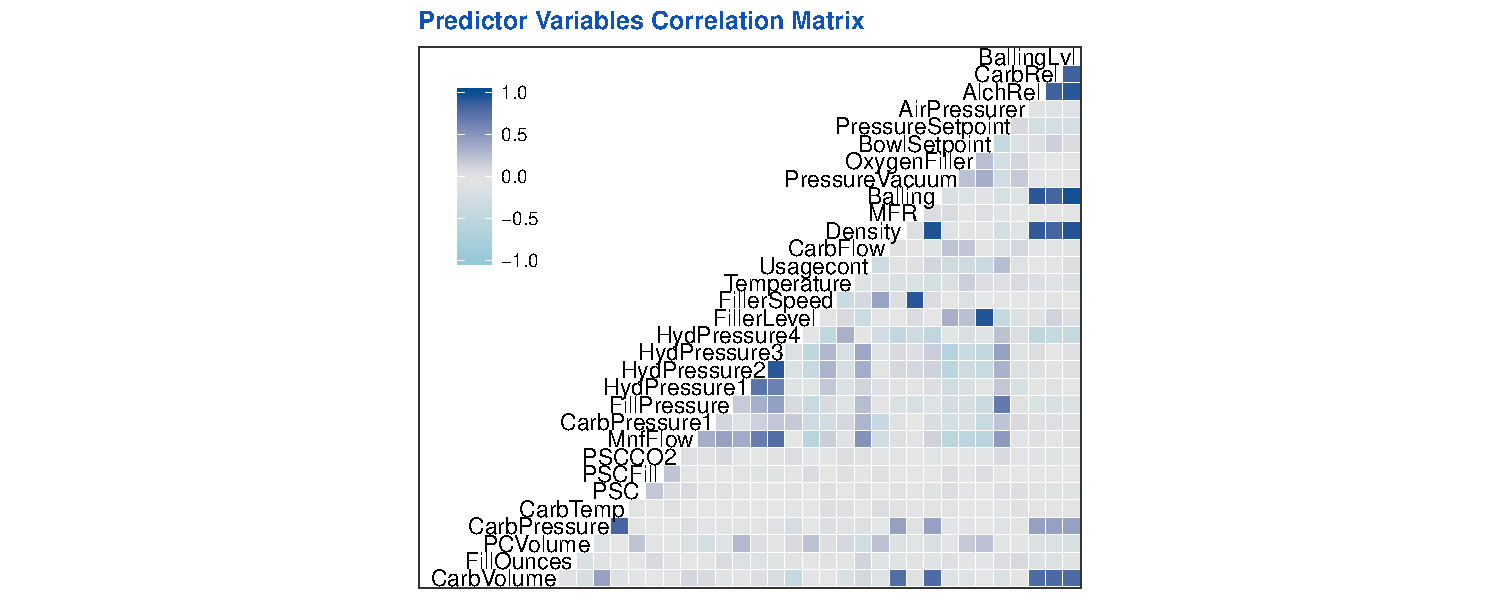
\includegraphics{Proj2-AndyHwang_files/figure-latex/unnamed-chunk-8-1} \end{center}

\subsection{Bivariate relationships}\label{bivariate-relationships}

Note that when \texttt{Oxygen\ Filler} has fairly positive relationship
with \texttt{PH}, \texttt{Temparature} has negative relationship. We
confirmed the relationships between predictors and target variable.

\begin{center}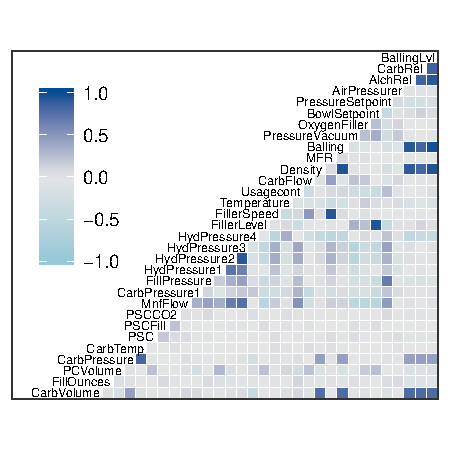
\includegraphics{Proj2-AndyHwang_files/figure-latex/unnamed-chunk-9-1} \end{center}

\subsection{Correlation Matrix}\label{correlation-matrix}

We confirmed that there are several highly correlated predictors. This
is another reason why \texttt{Random\ Forest} would be more preferred to
\texttt{Bagged\ Tree} model. In fact, \texttt{Random\ Forest} is more
robust to strong correlation than \texttt{Bagged\ Tree}. Although
multicollinearity is not a big problem for for \texttt{PLS} and
\texttt{Random\ Forest}, it can cause some problem when it comes to
inferring the importance of certain predictors in tree model.
Multicollinearity means that some predictors are shown as highly
correlated with other combincations of predictors in variable
importance. According to the reference, it may mislead business audience
to think that some features are not more important than others
vice-versa. However, we really do not know whether the reader of this
paper would still treat highly correlated variable such as
\texttt{HydPressure3} different from \texttt{HydPressure2} or not. Thus,
we will just keep the variables as they are.

Reference:

(``For example, the two surface area predictors have an extremely high
correlation (0.96) and each is used in the tree shown in Fig. 8.4. It is
possible that the small difference between these predictors is strongly
driving the choice between the two, but it is more likely to be due to
small, random differences in the variables. Because of this, more
predictors may be selected than actually needed. In addition, the
variable importance values are affected. If the solubility data only
contained one of the surface area predictors, then this predictor would
have likely been used twice in the tree, therefore inflating its
importance value. Instead, including both surface area predictors in the
data causes their importance to have only moderate values.'' Page 181 of
Applied Predictive Modeling - Max KJ)

\begin{center}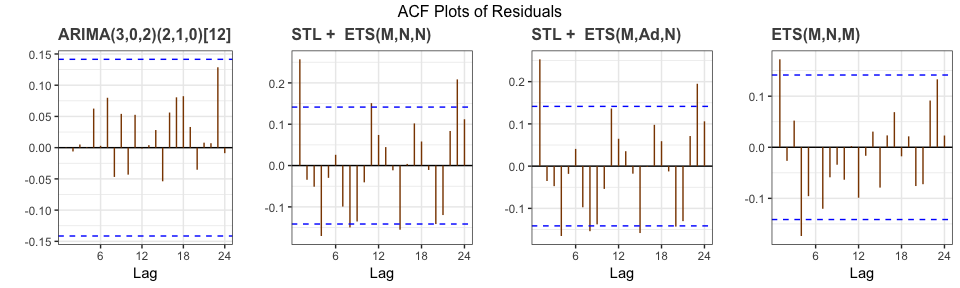
\includegraphics{Proj2-AndyHwang_files/figure-latex/unnamed-chunk-10-1} \end{center}

\chapter{Data preparation}\label{data-preparation}

Before modeling can be done, the issues identified during the data
exploration, namely, zero variance predictors, outliers and missing data
need to be addressed. For \texttt{BACON} (outlier handling method)
approach, categorical variable needs to be converted to numeric.

\section{Imputation}\label{imputation}

After reviewing a few methods of multiple imputation techniques,
Multiple Imputation Chained Equations (MICE) was selected for its
strength in handling imputation for observations with more than one
predictor missing. For categorical variable such as \texttt{Brand\ Code}
will be imputed by mode. For \texttt{BACON} to work, we will also
convert \texttt{Brand\ Code} to numeric.

We will also remove zero variance Predictors using \texttt{nearZeroVar}.
It diagnoses predictors that have one unique value (i.e.~are zero
variance predictors) or predictors that are have both of the following
characteristics: they have very few unique values relative to the number
of samples and the ratio of the frequency of the most common value to
the frequency of the second most common value is large.

For outlier handling, \texttt{BACON} is used. \texttt{BACON}, short for
`Blocked Adaptive Computationally-Efficient Outlier Nominators', is a
somewhat robust algorithm (set), with an implementation for regression
or multivariate covariance estimation. The function produces index with
\texttt{TRUE} or \texttt{FALSE} to identify rows with outliers. This
index will be used as \texttt{subset} to train outlier free train set in
the process of hyper-parameter tuning in \texttt{train} function and
train the final model using full train set without removing outliers
after being applied with best hyper-parameters.

\chapter{Modeling}\label{modeling}

\section{Model 1: Bagged Tree with
BACON}\label{model-1-bagged-tree-with-bacon}

\begin{table}[H]

\caption{\label{tab:unnamed-chunk-12}Model Summary - Bagged Tree with BACON}
\centering
\fontsize{8}{10}\selectfont
\begin{tabular}[t]{rrr}
\toprule
\textbf{RMSE} & \textbf{Rsquared} & \textbf{MAPE}\\
\midrule
\rowcolor{gray!6}  0.1198618 & 0.4922456 & 0.0106783\\
\bottomrule
\end{tabular}
\end{table}

\begin{center}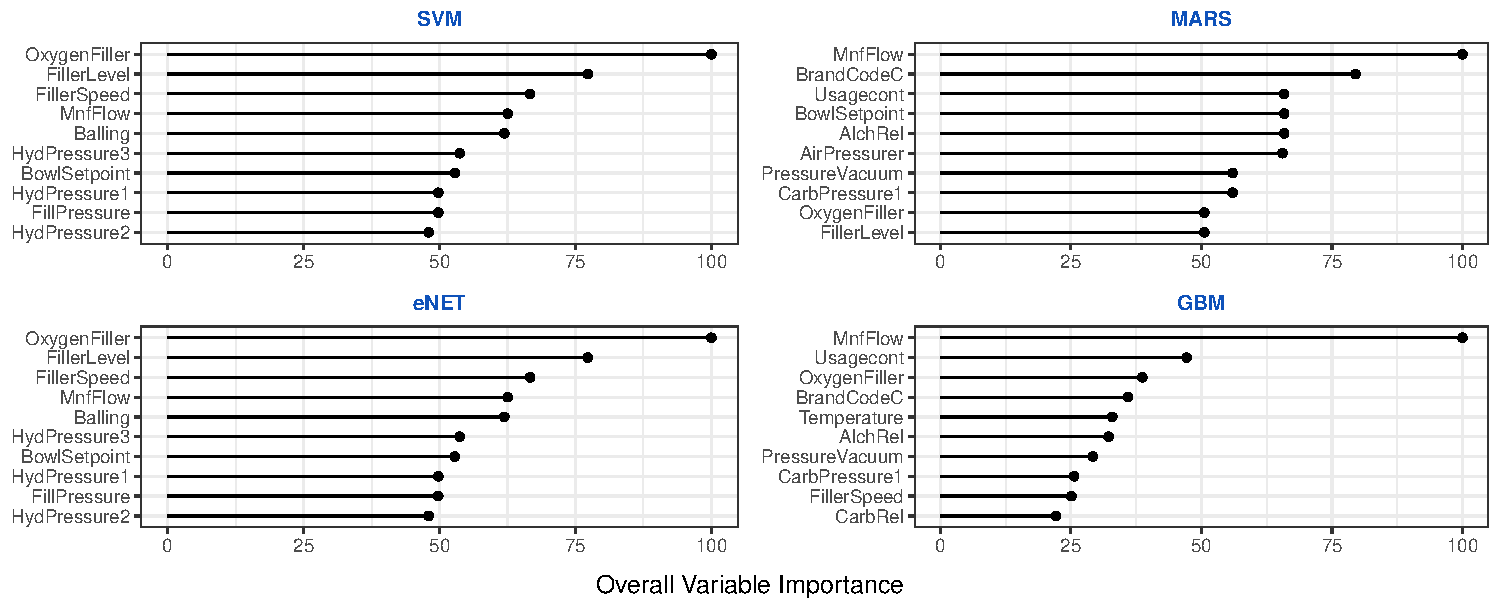
\includegraphics{Proj2-AndyHwang_files/figure-latex/unnamed-chunk-12-1} \end{center}

MAPE is 0.0106783 where as top 3 important predictors are
\texttt{CarbRel}, \texttt{OxygenFiler} and \texttt{Usuagecont}. Since
\texttt{Bagged\ Tree} uses all features for splitting a node Unlike
\texttt{Random\ Forest} which uses only a subset of features at random
out of the total for splitting each node in a tree, the order of feature
importances between two models can be quite different.

\section{Model 2: PLS with BACON}\label{model-2-pls-with-bacon}

\begin{table}[H]

\caption{\label{tab:unnamed-chunk-13}Model Summary - PLS with BACON}
\centering
\fontsize{8}{10}\selectfont
\begin{tabular}[t]{lrrr}
\toprule
\textbf{ } & \textbf{RMSE} & \textbf{Rsquared} & \textbf{MAPE}\\
\midrule
\rowcolor{gray!6}  10 & 0.1327207 & 0.3740444 & 0.0123968\\
\bottomrule
\end{tabular}
\end{table}

\begin{center}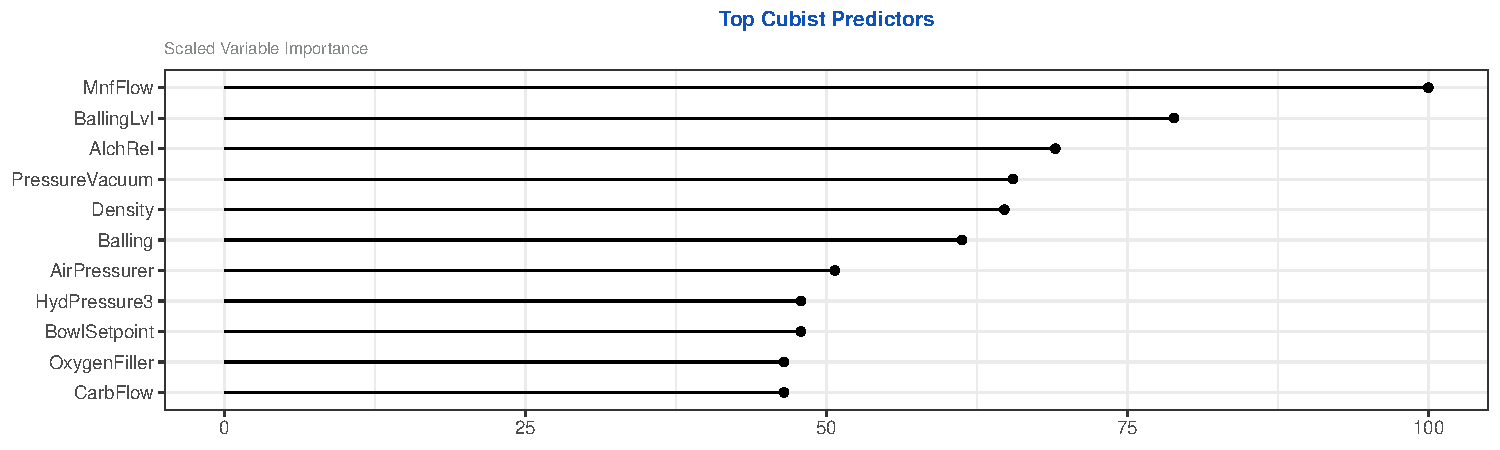
\includegraphics{Proj2-AndyHwang_files/figure-latex/unnamed-chunk-13-1} \end{center}

The final value used for the model was ncomp = 10. MAPE is 0.0123968,
0.0123968, 0.0123968, 0.0123968, 0.0123968, 0.0123968, 0.0123968,
0.0123968, 0.0123968, 0.0123968 where as top 3 important predictors are
\texttt{MnfFlow}, \texttt{Usuagecont} and \texttt{BowlSetpoint}. The
order of variable importance, again, is quite different from
\texttt{Bagged\ Tree} as \texttt{PLS} is not a tree-based model. Note
that PLS is a dimension reduction technique with some similarity to
principal component analysis. The predictor variables are mapped to a
smaller set of variables and within that smaller space we perform a
regression against the outcome variable. In contrast to principal
component analysis where the dimension reduction ignores the outcome
variable, the \texttt{PLS} procedure aims to choose new mapped variables
that maximally explain the outcome variable.

\section{Model 3: Random Forest with original data
set}\label{model-3-random-forest-with-original-data-set}

\begin{table}[H]

\caption{\label{tab:unnamed-chunk-15}Model Summary - RF with original data set}
\centering
\fontsize{8}{10}\selectfont
\begin{tabular}[t]{rrr}
\toprule
\textbf{RMSE} & \textbf{Rsquared} & \textbf{MAPE}\\
\midrule
\rowcolor{gray!6}  0.0969916 & 0.6909936 & 0.0081279\\
\bottomrule
\end{tabular}
\end{table}

\begin{center}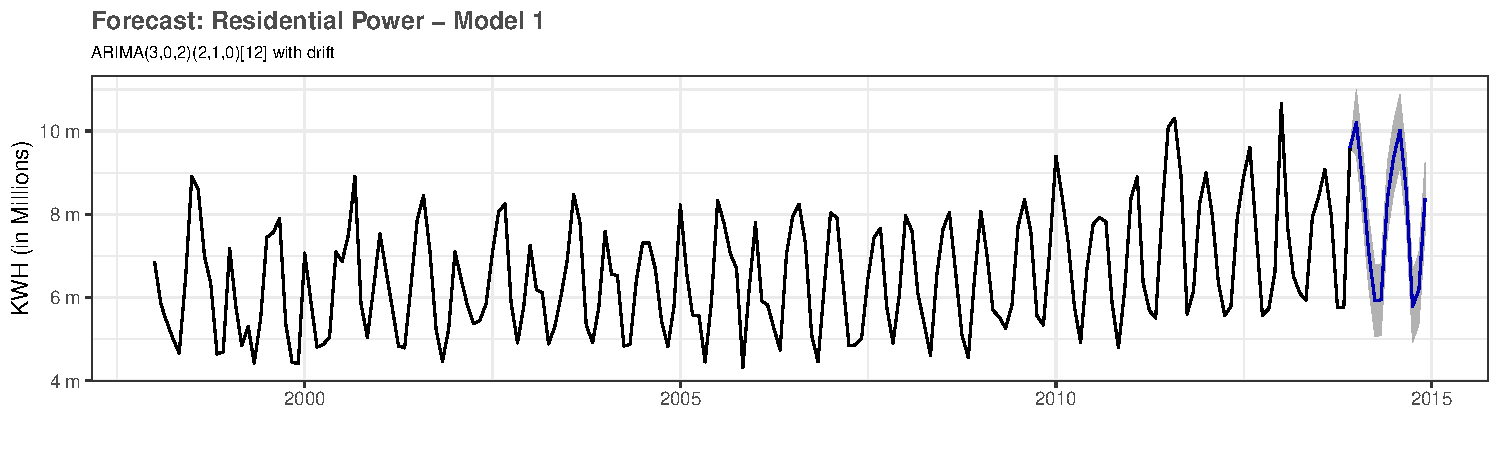
\includegraphics{Proj2-AndyHwang_files/figure-latex/unnamed-chunk-15-1} \end{center}

The final value used for the model was ncomp = 10. MAPE is 0.0081279
where as top 3 important predictors are \texttt{MnfFlow},
\texttt{BrandCode} and \texttt{PressureVacuum} for \%incMSE and
\texttt{MnfFlow}, \texttt{BrandCode} and \texttt{OxygenFiller} for
IncNodePurity. Unlike \texttt{PLS}, \texttt{Random\ Forest} can produce
2 different variable importance plots.

The first graph shows that if a variable is assigned values by random
permutation by how much will the MSE increase. The second plot is based
on \texttt{node\ purity} which is measured by \texttt{Gini\ Index} and
it is the the difference between RSS before and after the split on that
variable. In short, each graph shows how much MSE or Impurity increases
when each variable is randomly permuted.

\chapter{Evaluation}\label{evaluation}

\begin{table}[H]

\caption{\label{tab:unnamed-chunk-16}Evaluation Summary on test set}
\centering
\fontsize{8}{10}\selectfont
\begin{tabular}[t]{lrrr}
\toprule
\textbf{MODEL} & \textbf{RMSE} & \textbf{Rsquare} & \textbf{MAPE}\\
\midrule
\rowcolor{gray!6}  Bagged Tree & 0.1235554 & 0.5047507 & 0.0111408\\
PLS - BACON & 0.1358493 & 0.3862047 & 0.0122273\\
\rowcolor{gray!6}  RF & 0.0883145 & 0.7449339 & 0.0075050\\
\bottomrule
\end{tabular}
\end{table}

From the table, we confirmed that \texttt{Random\ Forest} is a clear
winner with the lowest MAPE on test set.

\section{Insight \& Conclusion}\label{insight-conclusion}

\begin{center}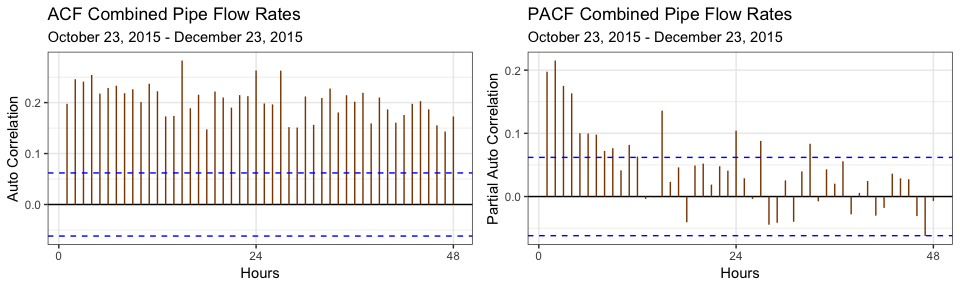
\includegraphics{Proj2-AndyHwang_files/figure-latex/unnamed-chunk-17-1} \end{center}

\begin{center}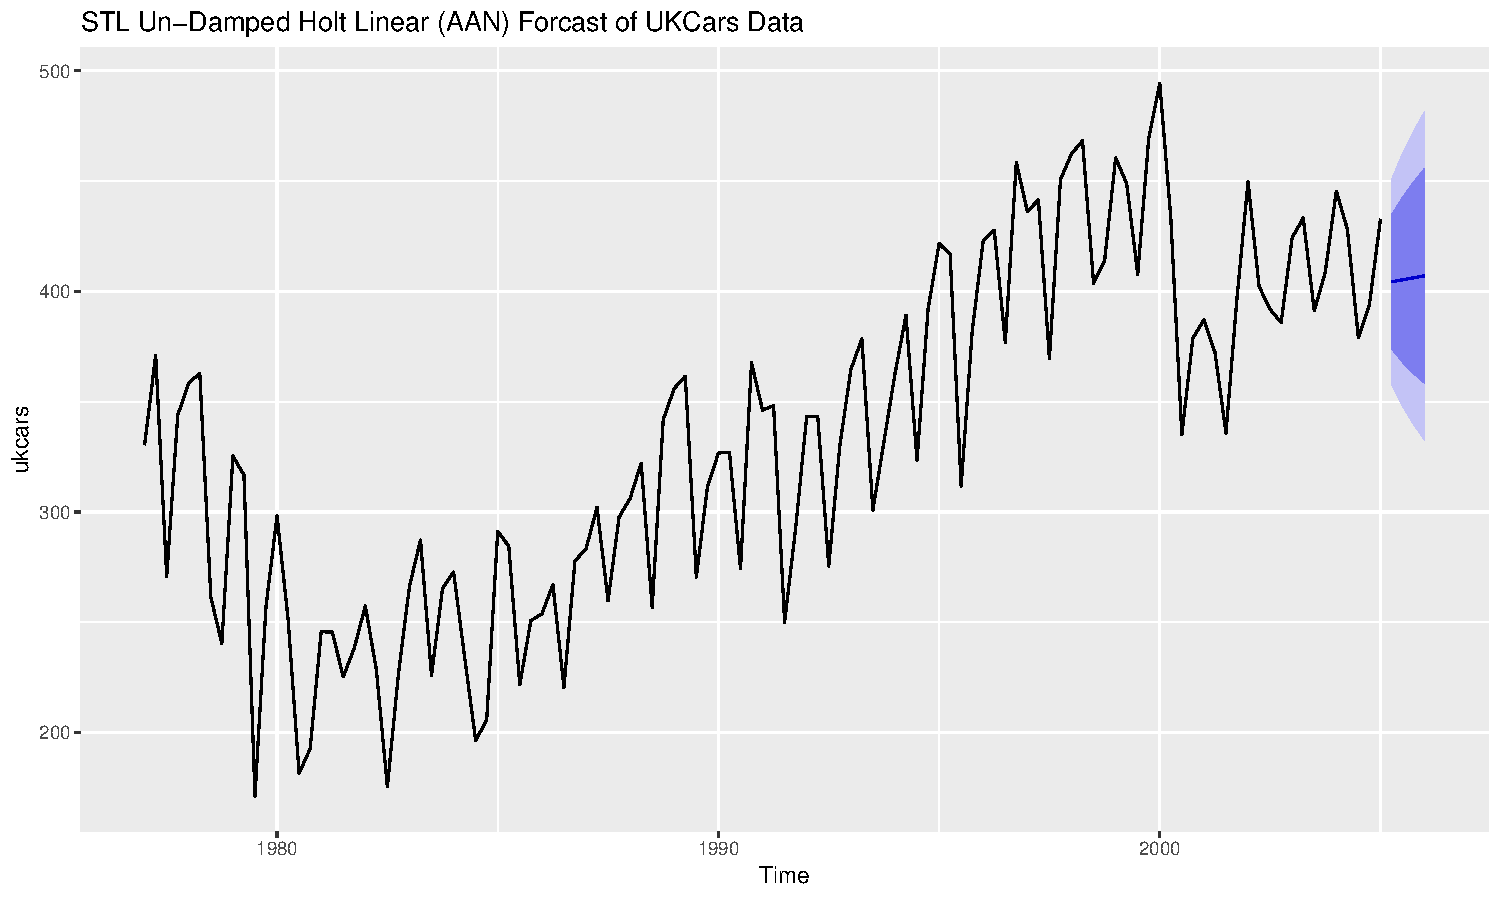
\includegraphics{Proj2-AndyHwang_files/figure-latex/unnamed-chunk-17-2} \end{center}

\begin{center}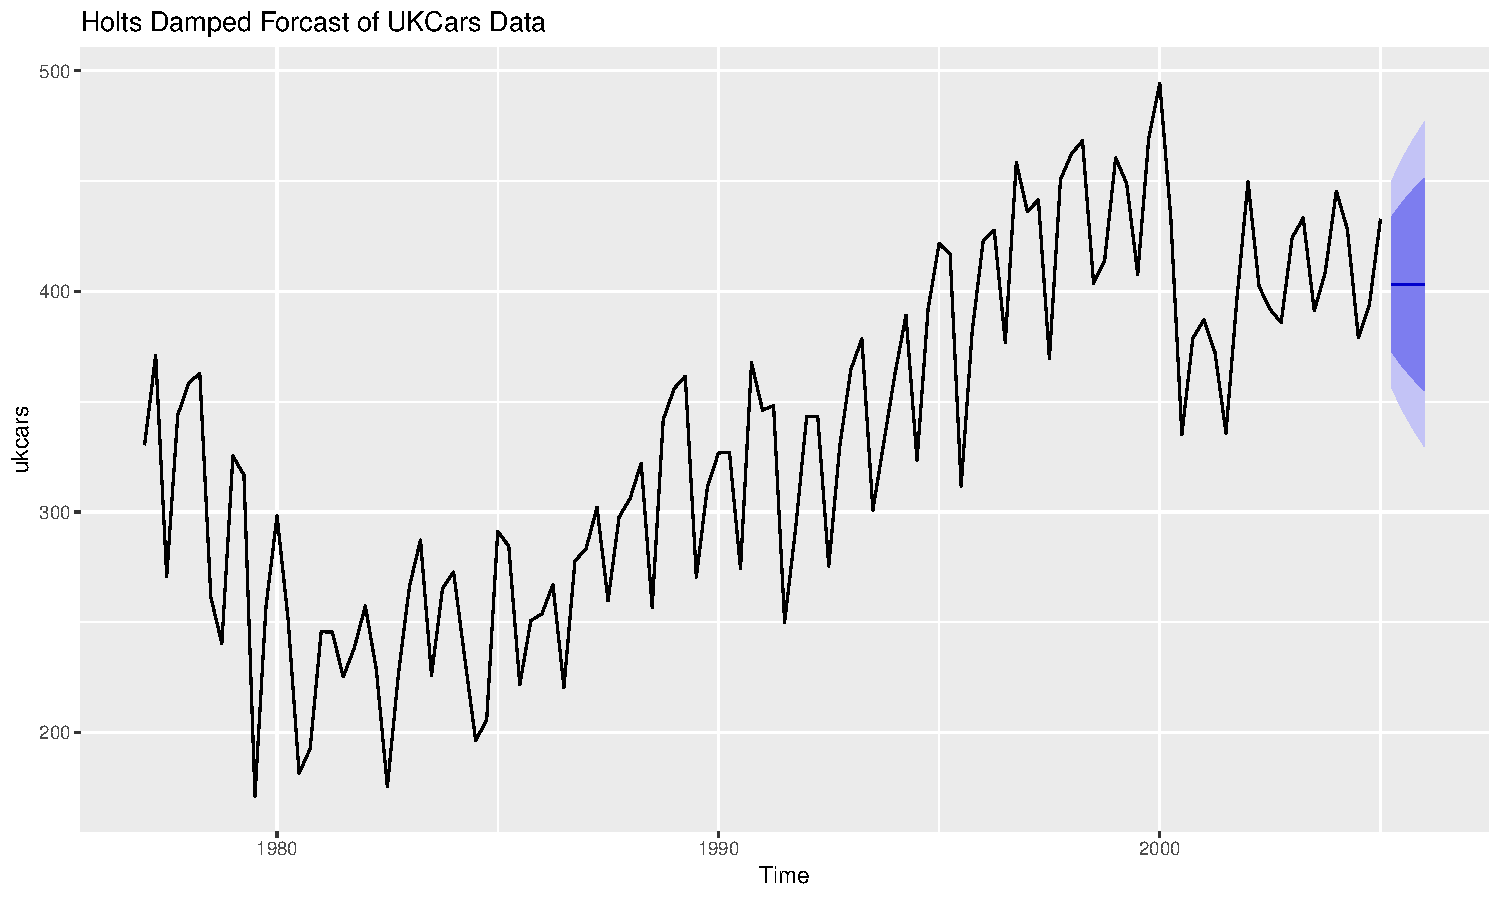
\includegraphics{Proj2-AndyHwang_files/figure-latex/unnamed-chunk-17-3} \end{center}

\begin{center}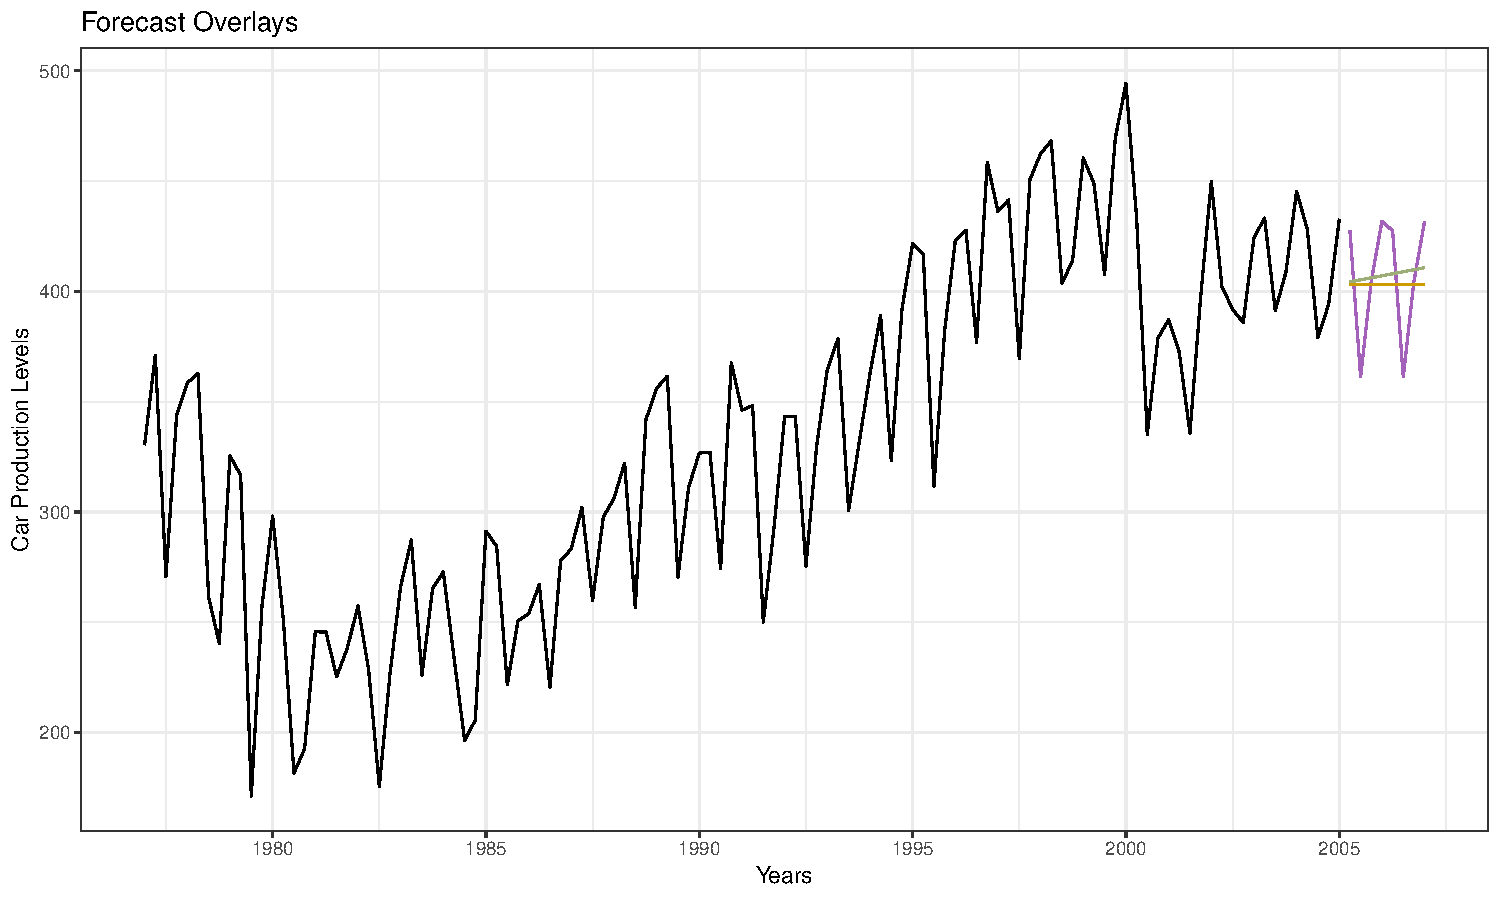
\includegraphics{Proj2-AndyHwang_files/figure-latex/unnamed-chunk-17-4} \end{center}

We graphed top 4 most important variables from \texttt{varImp} of MSE
and NodePurity. Given that \texttt{Brand\ Code} is categorical, we
grouped 3 continous variables into \texttt{Brand\ Code}.

The first feature plot shows that 3 continous variables have very weak
relationship with \texttt{PH}. \texttt{MnfFlow} has slight negative
relationship where as \texttt{PressureVacuum} and \texttt{OxygenFiller}
have slight positive relationship.

From grouping by \texttt{Brand\ Code}, we see that for \texttt{PH} vs
\texttt{MnfFlow} and \texttt{PH\ vs\ PressureVacuum}, it seems like
predictors have the most negative relationship with \texttt{PH} with
code = \texttt{B}. For \texttt{PH\ vs\ OxygenFiller}, code = \texttt{C}
seems to have the most negative relationship with \texttt{PH}.

We can recommend business users to put more attention on increasing
\texttt{MnfFlow} or decreasing \texttt{PressureVacuum} (especially code
= \texttt{B} for both) and \texttt{OxygenFiller} (especially code =
\texttt{C}) than any other predictors if their goal is to decrease
\texttt{PH}.

\section{Prediction}\label{prediction}

Let's export the prediction values of \texttt{Random\ Forest} (the best
model) on \texttt{StudentEvaluation} as CSV file.

\chapter*{Appendix}\label{Appendix}
\addcontentsline{toc}{chapter}{Appendix}

\begin{Shaded}
\begin{Highlighting}[]
\KeywordTok{library}\NormalTok{(tidyverse)}
\KeywordTok{library}\NormalTok{(readxl)}
\KeywordTok{library}\NormalTok{(psych)}
\KeywordTok{library}\NormalTok{(ggplot2)}
\KeywordTok{library}\NormalTok{(mice)}
\KeywordTok{library}\NormalTok{(xtable)}
\KeywordTok{library}\NormalTok{(GGally)}
\KeywordTok{library}\NormalTok{(ggstance)}
\KeywordTok{library}\NormalTok{(grid)}
\KeywordTok{library}\NormalTok{(gridExtra)}
\KeywordTok{library}\NormalTok{(ggpubr)}
\KeywordTok{library}\NormalTok{(caret)}
\KeywordTok{library}\NormalTok{(data.table)}
\KeywordTok{library}\NormalTok{(recipes)}
\KeywordTok{library}\NormalTok{(Metrics)}
\KeywordTok{library}\NormalTok{(randomForest)}
\KeywordTok{library}\NormalTok{(robustX)        }\CommentTok{# BACON}
\KeywordTok{library}\NormalTok{(ggcorrplot)     }\CommentTok{# Vis corr matrix}
\KeywordTok{library}\NormalTok{(e1071)          }\CommentTok{# Misc stats functions}

\NormalTok{df <-}\StringTok{ }\KeywordTok{read_excel}\NormalTok{(}\StringTok{'C:/Users/ahwang/Desktop/Cuny/DATA624/project2/data/StudentData.xlsx'}\NormalTok{)}
\NormalTok{df_eval <-}\StringTok{ }\KeywordTok{read_excel}\NormalTok{(}\StringTok{'C:/Users/ahwang/Desktop/Cuny/DATA624/project2/data/StudentEvaluation.xlsx'}\NormalTok{)}
\NormalTok{dict <-}\StringTok{ }\KeywordTok{read_excel}\NormalTok{(}\StringTok{'C:/Users/ahwang/Desktop/Cuny/DATA624/project2/data/DataDictionary.xlsx'}\NormalTok{)}

\CommentTok{# remove space in-between variable names}
\KeywordTok{colnames}\NormalTok{(df) <-}\StringTok{ }\KeywordTok{gsub}\NormalTok{(}\StringTok{" "}\NormalTok{,}\StringTok{""}\NormalTok{,}\KeywordTok{colnames}\NormalTok{(df))}

\CommentTok{# Introduction \{-#intro\}}

\CommentTok{# Data Exploration }
\NormalTok{## Data dictionary}

\KeywordTok{kable}\NormalTok{(dict, }\DataTypeTok{caption=}\StringTok{"Data dictionary"}\NormalTok{, }\DataTypeTok{booktabs=}\NormalTok{T)}\OperatorTok\KeywordTok{kable_styling}\NormalTok{()}\OperatorTok\KeywordTok{row_spec}\NormalTok{()}

\NormalTok{## Summary statistics}

\CommentTok{# Create a table summarizing the training data}
\CommentTok{# create lists of desired summary stats for calculation}
\NormalTok{statFuns <-}\StringTok{ }
\StringTok{  }\KeywordTok{funs}\NormalTok{(}\DataTypeTok{missing =} \KeywordTok{sum}\NormalTok{(}\KeywordTok{is.na}\NormalTok{(.))}
\NormalTok{       , }\DataTypeTok{min =} \KeywordTok{min}\NormalTok{(., }\DataTypeTok{na.rm =} \OtherTok{TRUE}\NormalTok{)}
\NormalTok{       , }\DataTypeTok{Q1 =} \KeywordTok{quantile}\NormalTok{(., .}\DecValTok{25}\NormalTok{, }\DataTypeTok{na.rm =} \OtherTok{TRUE}\NormalTok{)}
\NormalTok{       , }\DataTypeTok{mean =} \KeywordTok{mean}\NormalTok{(., }\DataTypeTok{na.rm =} \OtherTok{TRUE}\NormalTok{)}
\NormalTok{       , }\DataTypeTok{median =} \KeywordTok{median}\NormalTok{(., }\DataTypeTok{na.rm =} \OtherTok{TRUE}\NormalTok{)}
\NormalTok{       , }\DataTypeTok{Q3 =} \KeywordTok{quantile}\NormalTok{(., .}\DecValTok{75}\NormalTok{, }\DataTypeTok{na.rm =} \OtherTok{TRUE}\NormalTok{)}
\NormalTok{       , }\DataTypeTok{max =} \KeywordTok{max}\NormalTok{(., }\DataTypeTok{na.rm =} \OtherTok{TRUE}\NormalTok{)}
\NormalTok{       , }\DataTypeTok{sd =} \KeywordTok{sd}\NormalTok{(., }\DataTypeTok{na.rm =} \OtherTok{TRUE}\NormalTok{)}
\NormalTok{       , }\DataTypeTok{mad =} \KeywordTok{mad}\NormalTok{(., }\DataTypeTok{na.rm =} \OtherTok{TRUE}\NormalTok{)}
\NormalTok{       , }\DataTypeTok{skewness =} \KeywordTok{skewness}\NormalTok{(., }\DataTypeTok{na.rm =} \OtherTok{TRUE}\NormalTok{)}
\NormalTok{       , }\DataTypeTok{kurtosis =} \KeywordTok{kurtosis}\NormalTok{(., }\DataTypeTok{na.rm =} \OtherTok{TRUE}\NormalTok{)}
\NormalTok{  )}

\CommentTok{# Create data frame of basic summary stats}
\NormalTok{dfSumTrain  <-}\StringTok{ }
\StringTok{  }\NormalTok{df }\OperatorTok\StringTok{ }
\StringTok{  }\CommentTok{# union(dfEval %>% mutate(TARGET_WINS = as.numeric(NA))) %>% }
\StringTok{  }\NormalTok{dplyr}\OperatorTok{::}\KeywordTok{select}\NormalTok{(}\OperatorTok{-}\StringTok{`}\DataTypeTok{BrandCode}\StringTok{`}\NormalTok{) }\OperatorTok\StringTok{ }
\StringTok{  }\KeywordTok{summarise_all}\NormalTok{(statFuns) }\OperatorTok\StringTok{ }
\StringTok{  }\KeywordTok{gather}\NormalTok{() }\OperatorTok\StringTok{ }
\StringTok{  }\KeywordTok{separate}\NormalTok{(key, }\KeywordTok{c}\NormalTok{(}\StringTok{'metric'}\NormalTok{, }\StringTok{'stat'}\NormalTok{), }\DataTypeTok{sep =} \StringTok{'(_)(?!.*_)'}\NormalTok{) }\OperatorTok\StringTok{ }
\StringTok{  }\KeywordTok{spread}\NormalTok{(stat, value) }\OperatorTok\StringTok{ }
\StringTok{  }\NormalTok{dplyr}\OperatorTok{::}\KeywordTok{select}\NormalTok{(metric, }\KeywordTok{names}\NormalTok{(statFuns))}

\NormalTok{dfSumTrain }\OperatorTok\StringTok{ }\KeywordTok{kable}\NormalTok{(}\DataTypeTok{caption=}\StringTok{"Summary statistics"}\NormalTok{, }\DataTypeTok{booktabs=}\NormalTok{T)}\OperatorTok\KeywordTok{kable_styling}\NormalTok{()}\OperatorTok\KeywordTok{row_spec}\NormalTok{()}

\KeywordTok{table}\NormalTok{(df}\OperatorTok{$}\StringTok{`}\DataTypeTok{BrandCode}\StringTok{`}\NormalTok{, }\DataTypeTok{useNA =} \StringTok{"ifany"}\NormalTok{)}\OperatorTok\KeywordTok{kable}\NormalTok{(}\DataTypeTok{caption=}\StringTok{"Frequency distribution of BrandCode"}\NormalTok{, }\DataTypeTok{booktabs=}\NormalTok{T)}\OperatorTok\KeywordTok{kable_styling}\NormalTok{()}\OperatorTok\KeywordTok{row_spec}\NormalTok{()}

\NormalTok{## Visualizations}

\NormalTok{### Missing data}

\NormalTok{dfSumTrain }\OperatorTok\StringTok{ }
\StringTok{  }\KeywordTok{group_by}\NormalTok{(metric) }\OperatorTok\StringTok{ }
\StringTok{  }\KeywordTok{mutate}\NormalTok{(}\DataTypeTok{miss_perc =}\NormalTok{ missing }\OperatorTok{/}\StringTok{ }\OperatorTok{!!}\KeywordTok{nrow}\NormalTok{(df)) }\OperatorTok\StringTok{ }
\StringTok{  }\NormalTok{dplyr}\OperatorTok{::}\KeywordTok{select}\NormalTok{(metric,missing, miss_perc) }\OperatorTok\StringTok{ }
\StringTok{  }\KeywordTok{ggplot}\NormalTok{(}\DataTypeTok{data =}\NormalTok{ ., }\KeywordTok{aes}\NormalTok{(}\DataTypeTok{x =} \KeywordTok{reorder}\NormalTok{(metric, }\OperatorTok{-}\NormalTok{miss_perc) , }\DataTypeTok{y =}\NormalTok{ miss_perc)) }\OperatorTok{+}\StringTok{ }
\StringTok{  }\KeywordTok{geom_bar}\NormalTok{(}\DataTypeTok{stat =} \StringTok{'identity'}\NormalTok{) }\OperatorTok{+}
\StringTok{  }\KeywordTok{coord_flip}\NormalTok{() }\OperatorTok{+}\StringTok{ }
\StringTok{  }\KeywordTok{geom_text}\NormalTok{(}\KeywordTok{aes}\NormalTok{(}\DataTypeTok{label =}\NormalTok{ missing), }\DataTypeTok{hjust =} \OperatorTok{-}\FloatTok{0.1}\NormalTok{, }\DataTypeTok{size =} \DecValTok{3}\NormalTok{) }\OperatorTok{+}\StringTok{ }
\StringTok{  }\KeywordTok{labs}\NormalTok{(}\DataTypeTok{x =} \OtherTok{NULL}\NormalTok{, }\DataTypeTok{y =} \OtherTok{NULL}\NormalTok{, }\DataTypeTok{Title =} \StringTok{'% Missing'}\NormalTok{) }\OperatorTok{+}\StringTok{ }
\StringTok{  }\KeywordTok{theme_bw}\NormalTok{() }\OperatorTok{+}
\StringTok{  }\KeywordTok{theme}\NormalTok{(}\DataTypeTok{legend.position =} \StringTok{'none'}\NormalTok{) }\OperatorTok{+}\StringTok{ }
\StringTok{  }\KeywordTok{scale_y_continuous}\NormalTok{(}\DataTypeTok{labels =}\NormalTok{ scales}\OperatorTok{::}\NormalTok{percent)}

\NormalTok{### Univariate distributions}

\NormalTok{df }\OperatorTok\StringTok{ }
\StringTok{  }\CommentTok{# union(dfEval %>% mutate(TARGET_WINS = as.numeric(NA))) %>%}
\StringTok{  }\NormalTok{dplyr}\OperatorTok{::}\KeywordTok{select}\NormalTok{(}\OperatorTok{-}\NormalTok{BrandCode) }\OperatorTok\StringTok{ }
\StringTok{  }\KeywordTok{gather}\NormalTok{() }\OperatorTok\StringTok{ }
\StringTok{  }\KeywordTok{group_by}\NormalTok{(key) }\OperatorTok\StringTok{ }
\StringTok{  }\KeywordTok{ggplot}\NormalTok{(}\DataTypeTok{data =}\NormalTok{ ., }\KeywordTok{aes}\NormalTok{(value)) }\OperatorTok{+}\StringTok{ }
\StringTok{  }\KeywordTok{geom_histogram}\NormalTok{(}\DataTypeTok{bins =} \DecValTok{30}\NormalTok{, }\KeywordTok{aes}\NormalTok{(}\DataTypeTok{y =}\NormalTok{ ..density..)) }\OperatorTok{+}
\StringTok{  }\KeywordTok{geom_density}\NormalTok{(}\DataTypeTok{alpha =} \FloatTok{0.3}\NormalTok{, }\DataTypeTok{color =} \OtherTok{NA}\NormalTok{, }\DataTypeTok{fill =} \StringTok{'lightgreen'}\NormalTok{) }\OperatorTok{+}\StringTok{ }
\StringTok{  }\KeywordTok{scale_x_continuous}\NormalTok{(}\DataTypeTok{labels =}\NormalTok{ scales}\OperatorTok{::}\NormalTok{comma) }\OperatorTok{+}
\StringTok{  }\KeywordTok{scale_y_continuous}\NormalTok{(}\DataTypeTok{labels =}\NormalTok{ scales}\OperatorTok{::}\NormalTok{percent) }\OperatorTok{+}
\StringTok{  }\KeywordTok{facet_wrap}\NormalTok{(}\OperatorTok{~}\NormalTok{key, }\DataTypeTok{scales =} \StringTok{'free'}\NormalTok{) }\OperatorTok{+}\StringTok{ }
\StringTok{  }\KeywordTok{labs}\NormalTok{(}\DataTypeTok{x =} \OtherTok{NULL}\NormalTok{, }\DataTypeTok{y =} \OtherTok{NULL}\NormalTok{) }\OperatorTok{+}\StringTok{ }
\StringTok{  }\KeywordTok{theme_bw}\NormalTok{() }\OperatorTok{+}
\StringTok{  }\KeywordTok{theme}\NormalTok{(}\DataTypeTok{axis.text.x =} \KeywordTok{element_text}\NormalTok{(}\DataTypeTok{angle =} \DecValTok{30}\NormalTok{, }\DataTypeTok{hjust =} \DecValTok{1}\NormalTok{))}

\NormalTok{df }\OperatorTok\StringTok{ }
\StringTok{  }\CommentTok{# union(dfEval %>% mutate(TARGET_WINS = as.numeric(NA))) %>%}
\StringTok{  }\NormalTok{dplyr}\OperatorTok{::}\KeywordTok{select}\NormalTok{(}\OperatorTok{-}\NormalTok{BrandCode) }\OperatorTok\StringTok{ }
\StringTok{  }\KeywordTok{gather}\NormalTok{() }\OperatorTok\StringTok{ }
\StringTok{  }\KeywordTok{group_by}\NormalTok{(key) }\OperatorTok\StringTok{ }
\StringTok{  }\KeywordTok{ggplot}\NormalTok{(}\DataTypeTok{data =}\NormalTok{ ., }\KeywordTok{aes}\NormalTok{(}\DataTypeTok{x =} \StringTok{''}\NormalTok{, }\DataTypeTok{y =}\NormalTok{ value)) }\OperatorTok{+}\StringTok{ }
\StringTok{  }\KeywordTok{geom_boxplot}\NormalTok{() }\OperatorTok{+}\StringTok{ }
\StringTok{  }\KeywordTok{geom_violin}\NormalTok{(}\DataTypeTok{alpha =} \FloatTok{0.3}\NormalTok{, }\DataTypeTok{color =} \OtherTok{NA}\NormalTok{, }\DataTypeTok{fill =} \StringTok{'lightgreen'}\NormalTok{) }\OperatorTok{+}\StringTok{ }
\StringTok{  }\KeywordTok{labs}\NormalTok{(}\DataTypeTok{x =} \OtherTok{NULL}\NormalTok{, }\DataTypeTok{y =} \OtherTok{NULL}\NormalTok{) }\OperatorTok{+}\StringTok{ }
\StringTok{  }\KeywordTok{theme_bw}\NormalTok{() }\OperatorTok{+}
\StringTok{  }\KeywordTok{theme}\NormalTok{(}\DataTypeTok{axis.ticks.y=}\KeywordTok{element_blank}\NormalTok{()) }\OperatorTok{+}\StringTok{ }
\StringTok{  }\KeywordTok{facet_wrap}\NormalTok{(}\OperatorTok{~}\NormalTok{key, }\DataTypeTok{scales =} \StringTok{'free'}\NormalTok{, }\DataTypeTok{ncol =} \DecValTok{2}\NormalTok{) }\OperatorTok{+}\StringTok{ }
\StringTok{  }\KeywordTok{coord_flip}\NormalTok{()}

\NormalTok{### Bivariate relationships }

\NormalTok{df }\OperatorTok\StringTok{ }
\StringTok{  }\NormalTok{dplyr}\OperatorTok{::}\KeywordTok{select}\NormalTok{(}\OperatorTok{-}\NormalTok{BrandCode) }\OperatorTok\StringTok{ }
\StringTok{  }\KeywordTok{gather}\NormalTok{(key, value, }\OperatorTok{-}\NormalTok{PH) }\OperatorTok\StringTok{ }
\StringTok{  }\KeywordTok{group_by}\NormalTok{(key) }\OperatorTok\StringTok{ }
\StringTok{  }\KeywordTok{ggplot}\NormalTok{(}\DataTypeTok{data =}\NormalTok{ ., }\KeywordTok{aes}\NormalTok{(}\DataTypeTok{x =}\NormalTok{ value, }\DataTypeTok{y =}\NormalTok{ PH)) }\OperatorTok{+}\StringTok{ }
\StringTok{  }\KeywordTok{geom_point}\NormalTok{() }\OperatorTok{+}\StringTok{ }
\StringTok{  }\KeywordTok{geom_smooth}\NormalTok{(}\DataTypeTok{method =} \StringTok{'gam'}\NormalTok{) }\OperatorTok{+}\StringTok{ }
\StringTok{  }\KeywordTok{facet_wrap}\NormalTok{(}\OperatorTok{~}\NormalTok{key, }\DataTypeTok{scales =} \StringTok{'free'}\NormalTok{) }\OperatorTok{+}\StringTok{ }
\StringTok{  }\KeywordTok{labs}\NormalTok{(}\DataTypeTok{x =} \OtherTok{NULL}\NormalTok{) }\OperatorTok{+}\StringTok{ }
\StringTok{  }\KeywordTok{theme_bw}\NormalTok{() }\OperatorTok{+}
\StringTok{  }\KeywordTok{theme}\NormalTok{(}\DataTypeTok{axis.text.x =} \KeywordTok{element_text}\NormalTok{(}\DataTypeTok{angle =} \DecValTok{30}\NormalTok{, }\DataTypeTok{hjust =} \DecValTok{1}\NormalTok{))}

\NormalTok{### Correlation Matrix}

\CommentTok{# Calculate pairwise pearson correlation and display as upper matrix plot}
\NormalTok{df }\OperatorTok\StringTok{ }
\StringTok{  }\CommentTok{# union(dfEval %>% mutate(TARGET_WINS = as.numeric(NA))) %>%}
\StringTok{  }\NormalTok{dplyr}\OperatorTok{::}\KeywordTok{select}\NormalTok{(}\OperatorTok{-}\KeywordTok{c}\NormalTok{(}\StringTok{'BrandCode'}\NormalTok{,}\StringTok{'PH'}\NormalTok{)) }\OperatorTok\StringTok{ }
\StringTok{  }\KeywordTok{cor}\NormalTok{(}\DataTypeTok{method =} \StringTok{'pearson'}\NormalTok{, }\DataTypeTok{use =} \StringTok{'pairwise.complete.obs'}\NormalTok{) }\OperatorTok\StringTok{ }
\StringTok{  }\KeywordTok{ggcorrplot}\NormalTok{(}\DataTypeTok{corr =}\NormalTok{ ., }\DataTypeTok{method =} \StringTok{'square'}\NormalTok{, }\DataTypeTok{type =} \StringTok{'upper'}
\NormalTok{             , }\DataTypeTok{lab =} \OtherTok{TRUE}\NormalTok{, }\DataTypeTok{lab_size =} \DecValTok{3}\NormalTok{, }\DataTypeTok{lab_col =} \StringTok{'grey20'}\NormalTok{)}

\CommentTok{# Data preparation}
\NormalTok{## Imputation}

\CommentTok{# set seed for split to allow for reproducibility}
\KeywordTok{set.seed}\NormalTok{(}\DecValTok{58677}\NormalTok{)}

\CommentTok{# use mice w/ default settings to impute missing data}
\NormalTok{miceImput <-}\StringTok{ }\KeywordTok{mice}\NormalTok{(df, }\DataTypeTok{printFlag =} \OtherTok{FALSE}\NormalTok{)}

\CommentTok{# add imputed data to original data set}
\NormalTok{df_mice <-}\StringTok{ }\KeywordTok{complete}\NormalTok{(miceImput)}
\NormalTok{df_mice}\OperatorTok{$}\NormalTok{BrandCode[}\KeywordTok{is.na}\NormalTok{(df_mice}\OperatorTok{$}\NormalTok{BrandCode)] <-}\StringTok{ 'B'}
\CommentTok{#table(df_mice$BrandCode, useNA = "ifany")}

\CommentTok{# Look for any features with no variance:}
\NormalTok{zero_cols <-}\StringTok{ }\KeywordTok{nearZeroVar}\NormalTok{( df_mice )}
\NormalTok{df_final <-}\StringTok{ }\NormalTok{df_mice[,}\OperatorTok{-}\NormalTok{zero_cols] }\CommentTok{# drop these zero variance columns }
\NormalTok{df_final}\OperatorTok{$}\NormalTok{BrandCode <-}\StringTok{ }\KeywordTok{as.factor}\NormalTok{(df_final}\OperatorTok{$}\NormalTok{BrandCode)}

\CommentTok{# convert categorical factor into numeric}
\NormalTok{M <-}\StringTok{ }\NormalTok{df_final}
\NormalTok{must_convert<-}\KeywordTok{sapply}\NormalTok{(M,is.factor) }\CommentTok{# logical vector telling if a variable needs to be displayed as numeric}
\NormalTok{BrandNumeric <-}\StringTok{ }\KeywordTok{sapply}\NormalTok{(M[,must_convert],unclass)    }\CommentTok{# data.frame of all categorical variables now displayed as numeric}
\NormalTok{df_final2<-}\KeywordTok{cbind}\NormalTok{(M[,}\OperatorTok{!}\NormalTok{must_convert],BrandNumeric)        }\CommentTok{# complete data.frame with all variables put together}

\CommentTok{# split data train/test}
\CommentTok{# df for random forest}
\NormalTok{training <-}\StringTok{ }\NormalTok{df_final}\OperatorTok{$}\NormalTok{PH }\OperatorTok\KeywordTok{createDataPartition}\NormalTok{(}\DataTypeTok{p =} \FloatTok{0.8}\NormalTok{, }\DataTypeTok{list =} \OtherTok{FALSE}\NormalTok{)}
\NormalTok{df_train <-}\StringTok{ }\NormalTok{df_final[training, ]}
\NormalTok{df_test <-}\StringTok{ }\NormalTok{df_final[}\OperatorTok{-}\NormalTok{training, ]}

\CommentTok{# df for PLS and Bagging}
\NormalTok{training2 <-}\StringTok{ }\NormalTok{df_final2}\OperatorTok{$}\NormalTok{PH }\OperatorTok\KeywordTok{createDataPartition}\NormalTok{(}\DataTypeTok{p =} \FloatTok{0.8}\NormalTok{, }\DataTypeTok{list =} \OtherTok{FALSE}\NormalTok{)}
\NormalTok{df_train2 <-}\StringTok{ }\NormalTok{df_final2[training2, ]}
\NormalTok{df_test2 <-}\StringTok{ }\NormalTok{df_final2[}\OperatorTok{-}\NormalTok{training2, ]}

\CommentTok{# X and y split for BACON fit}
\NormalTok{x <-}\StringTok{ }\KeywordTok{subset}\NormalTok{(df_train2, }\DataTypeTok{select =} \OperatorTok{-}\KeywordTok{c}\NormalTok{(PH) )}
\NormalTok{x <-}\StringTok{ }\KeywordTok{as.matrix}\NormalTok{(x)}
\NormalTok{y <-}\StringTok{ }\NormalTok{df_train2[, }\KeywordTok{c}\NormalTok{(}\StringTok{'PH'}\NormalTok{)]}

\NormalTok{bacon_fit <-}\StringTok{ }\KeywordTok{BACON}\NormalTok{(}\DataTypeTok{x =}\NormalTok{ x, }\DataTypeTok{y =}\NormalTok{ y)}

\CommentTok{# Modeling}

\NormalTok{## Model 1: Bagged Tree with BACON}

\KeywordTok{set.seed}\NormalTok{(}\DecValTok{58677}\NormalTok{)}
\NormalTok{bagged_model <-}\StringTok{ }\KeywordTok{train}\NormalTok{( PH}\OperatorTok{~}\NormalTok{., }\DataTypeTok{data =}\NormalTok{ df_train2, }\DataTypeTok{method=}\StringTok{"treebag"}\NormalTok{,}
                       \DataTypeTok{tuneLength=}\DecValTok{10}\NormalTok{, }
                       \DataTypeTok{subset =}\NormalTok{ bacon_fit}\OperatorTok{$}\NormalTok{subset,}
                       \DataTypeTok{trControl=}\KeywordTok{trainControl}\NormalTok{(}\DataTypeTok{method=}\StringTok{"cv"}\NormalTok{,}\DataTypeTok{number=}\DecValTok{5}\NormalTok{) )}

\CommentTok{# create MAPE table}
\NormalTok{train_bag_pred <-}\StringTok{ }\KeywordTok{predict}\NormalTok{(bagged_model)}
\NormalTok{bagged_model}\OperatorTok{$}\NormalTok{results}\OperatorTok{$}\NormalTok{MAPE <-}\StringTok{ }\NormalTok{Metrics}\OperatorTok{::}\KeywordTok{mape}\NormalTok{(df_train2}\OperatorTok{$}\NormalTok{PH, train_bag_pred)}

\NormalTok{bagged_model}\OperatorTok{$}\NormalTok{results[,}\KeywordTok{c}\NormalTok{(}\DecValTok{2}\NormalTok{,}\DecValTok{3}\NormalTok{,}\DecValTok{8}\NormalTok{)]}\OperatorTok\KeywordTok{kable}\NormalTok{(}\DataTypeTok{caption=}\StringTok{"Model Summary - Bagged Tree with BACON"}\NormalTok{, }\DataTypeTok{booktabs=}\NormalTok{T)}\OperatorTok\KeywordTok{kable_styling}\NormalTok{()}\OperatorTok\KeywordTok{row_spec}\NormalTok{()}

\CommentTok{# plot varImp}
\KeywordTok{plot}\NormalTok{(}\KeywordTok{varImp}\NormalTok{(bagged_model))}

\NormalTok{## Model 2: PLS with BACON}

\KeywordTok{set.seed}\NormalTok{(}\DecValTok{58677}\NormalTok{)}
\NormalTok{df_final2}\OperatorTok{$}\NormalTok{BrandNumeric <-}\StringTok{ }\KeywordTok{as.factor}\NormalTok{(df_final2}\OperatorTok{$}\NormalTok{BrandNumeric)}

\NormalTok{pls_model <-}\StringTok{ }\KeywordTok{train}\NormalTok{( PH}\OperatorTok{~}\NormalTok{., }\DataTypeTok{data =}\NormalTok{ df_train2, }\DataTypeTok{method=}\StringTok{"pls"}\NormalTok{,}
                    \DataTypeTok{tuneLength=}\DecValTok{10}\NormalTok{, }
                    \DataTypeTok{subset =}\NormalTok{ bacon_fit}\OperatorTok{$}\NormalTok{subset,}
                    \DataTypeTok{preProcess=}\KeywordTok{c}\NormalTok{(}\StringTok{"center"}\NormalTok{,}\StringTok{"scale"}\NormalTok{), }\DataTypeTok{trControl=}\KeywordTok{trainControl}\NormalTok{(}\DataTypeTok{method=}\StringTok{"cv"}\NormalTok{,}\DataTypeTok{number=}\DecValTok{5}\NormalTok{) )}

\CommentTok{# create MAPE table}
\NormalTok{train_pls_pred <-}\StringTok{ }\KeywordTok{predict}\NormalTok{(pls_model)}
\NormalTok{pls_model}\OperatorTok{$}\NormalTok{results}\OperatorTok{$}\NormalTok{MAPE <-}\StringTok{ }\NormalTok{Metrics}\OperatorTok{::}\KeywordTok{mape}\NormalTok{(df_train2}\OperatorTok{$}\NormalTok{PH, train_pls_pred)}

\NormalTok{pls_model}\OperatorTok{$}\NormalTok{results[}\DecValTok{10}\NormalTok{,}\KeywordTok{c}\NormalTok{(}\DecValTok{2}\NormalTok{,}\DecValTok{3}\NormalTok{,}\DecValTok{8}\NormalTok{)]}\OperatorTok\KeywordTok{kable}\NormalTok{(}\DataTypeTok{caption=}\StringTok{"Model Summary - PLS with BACON"}\NormalTok{, }\DataTypeTok{booktabs=}\NormalTok{T)}\OperatorTok\KeywordTok{kable_styling}\NormalTok{()}\OperatorTok\KeywordTok{row_spec}\NormalTok{()}

\CommentTok{# plot varImp}
\KeywordTok{plot}\NormalTok{(}\KeywordTok{varImp}\NormalTok{(pls_model))}

\NormalTok{## Model 3-1: Random Forest with BACON}

\CommentTok{# set.seed(58677)}
\CommentTok{# rf_model <- train( PH~., data = df_train2, method="rf",}
\CommentTok{#                    tuneLength=10, }
\CommentTok{#                    subset = bacon_fit$subset,}
\CommentTok{#                    importance = TRUE,}
\CommentTok{#                    trControl=trainControl(method="cv",number=5) )}
\CommentTok{# }
\CommentTok{# # create MAPE table}
\CommentTok{# train_rf_pred <- predict(rf_model)}
\CommentTok{# rf_model$results$MAPE <- Metrics::mape(df_train2$PH, train_rf_pred)}
\CommentTok{# }
\CommentTok{# rf_model$results%>%kable(caption="Model Summary - RF with BACON", booktabs=T)%>%kable_styling()%>%row_spec()}
\CommentTok{# }
\CommentTok{# # plot varImp}
\CommentTok{# plot(varImp(rf_model))}
\CommentTok{# }
\CommentTok{# Although `BACON` is not needed for `Random Forest`, it would not bother using it anyway. We will expermient the effect of `BACON` in `Random Forest`. The final value used for the model was ncomp = 10. MAPE is `r rf_model$results$MAPE` where as top 3 important predictors are `MnfFlow`, `Usuagecont` and `BowlSetpoint`. }

\NormalTok{## Model 3: Random Forest with original data set}

\KeywordTok{set.seed}\NormalTok{(}\DecValTok{58677}\NormalTok{)}

\CommentTok{# Algorithm Tune (tuneRF)}
\CommentTok{#bestmtry <- tuneRF(df_train[, -25], df_train[,25], stepFactor=1.5, improve=1e-5, ntree=2500)}

\NormalTok{##mtry <- ( (ncol(df_train) -1) / 3 ) or sqrt(ncol(df_train) - 1) # By default, # of predictors / 3 for regression, sqrt(# of predictors) for classification https://www.hackerearth.com/practice/machine-learning/machine-learning-algorithms/tutorial-random-forest-parameter-tuning-r/tutorial/}

\CommentTok{# from above result, we got mtry= 27 and ntree=2500 as optimal parameters}
\NormalTok{rf_model2 <-}\StringTok{ }\KeywordTok{randomForest}\NormalTok{(PH}\OperatorTok{~}\NormalTok{., }\DataTypeTok{data=}\NormalTok{df_train, }\DataTypeTok{method=}\StringTok{"rf"}\NormalTok{, }\DataTypeTok{mtry=} \DecValTok{31}\NormalTok{, }\DataTypeTok{importance =} \OtherTok{TRUE}\NormalTok{, }\DataTypeTok{ntree =} \DecValTok{2500}\NormalTok{)}

\CommentTok{# create MAPE table}
\NormalTok{train_rf_pred2 <-}\StringTok{ }\KeywordTok{predict}\NormalTok{(rf_model2)}

\NormalTok{s <-}\StringTok{ }\KeywordTok{data.frame}\NormalTok{(}
  \DataTypeTok{RMSE =}\NormalTok{ Metrics}\OperatorTok{::}\KeywordTok{rmse}\NormalTok{(df_train}\OperatorTok{$}\NormalTok{PH, train_rf_pred2),}
  \DataTypeTok{Rsquared =}\NormalTok{ caret}\OperatorTok{::}\KeywordTok{R2}\NormalTok{(df_train}\OperatorTok{$}\NormalTok{PH, train_rf_pred2),}
  \DataTypeTok{MAPE =}\NormalTok{ Metrics}\OperatorTok{::}\KeywordTok{mape}\NormalTok{(df_train}\OperatorTok{$}\NormalTok{PH, train_rf_pred2) )}

\NormalTok{s}\OperatorTok\KeywordTok{kable}\NormalTok{(}\DataTypeTok{caption=}\StringTok{"Model Summary - RF with original data set"}\NormalTok{, }\DataTypeTok{booktabs=}\NormalTok{T)}\OperatorTok\KeywordTok{kable_styling}\NormalTok{()}\OperatorTok\KeywordTok{row_spec}\NormalTok{()}

\CommentTok{# plot varImp}
\KeywordTok{varImpPlot}\NormalTok{(rf_model2)}

\CommentTok{# Evaluation}

\CommentTok{# Make predictions}
\NormalTok{p1 <-}\StringTok{ }\NormalTok{bagged_model }\OperatorTok\StringTok{ }\KeywordTok{predict}\NormalTok{(df_test2)}
\NormalTok{p2 <-}\StringTok{ }\NormalTok{pls_model }\OperatorTok\StringTok{ }\KeywordTok{predict}\NormalTok{(df_test2)}
\NormalTok{p3 <-}\StringTok{ }\NormalTok{rf_model2 }\OperatorTok\StringTok{ }\KeywordTok{predict}\NormalTok{(df_test)}

\CommentTok{# Model performance metrics}
\NormalTok{sum_t <-}\StringTok{ }\KeywordTok{data.frame}\NormalTok{(}
  \DataTypeTok{MODEL =} \KeywordTok{c}\NormalTok{(}\StringTok{'Bagged Tree'}\NormalTok{,}
            \StringTok{'PLS - BACON'}\NormalTok{,}
            \StringTok{'RF'}\NormalTok{),}
  \DataTypeTok{RMSE =} \KeywordTok{c}\NormalTok{(caret}\OperatorTok{::}\KeywordTok{RMSE}\NormalTok{(p1, df_test2}\OperatorTok{$}\NormalTok{PH),}
\NormalTok{           caret}\OperatorTok{::}\KeywordTok{RMSE}\NormalTok{(p2, df_test2}\OperatorTok{$}\NormalTok{PH),}
\NormalTok{           caret}\OperatorTok{::}\KeywordTok{RMSE}\NormalTok{(p3, df_test}\OperatorTok{$}\NormalTok{PH) ),}
  \DataTypeTok{Rsquare =} \KeywordTok{c}\NormalTok{(caret}\OperatorTok{::}\KeywordTok{R2}\NormalTok{(p1, df_test2}\OperatorTok{$}\NormalTok{PH),}
\NormalTok{              caret}\OperatorTok{::}\KeywordTok{R2}\NormalTok{(p2, df_test2}\OperatorTok{$}\NormalTok{PH),}
\NormalTok{              caret}\OperatorTok{::}\KeywordTok{R2}\NormalTok{(p3, df_test}\OperatorTok{$}\NormalTok{PH)),}
  \DataTypeTok{MAPE =} \KeywordTok{c}\NormalTok{(Metrics}\OperatorTok{::}\KeywordTok{mape}\NormalTok{(p1, df_test2}\OperatorTok{$}\NormalTok{PH),}
\NormalTok{           Metrics}\OperatorTok{::}\KeywordTok{mape}\NormalTok{(p2, df_test2}\OperatorTok{$}\NormalTok{PH),}
\NormalTok{           Metrics}\OperatorTok{::}\KeywordTok{mape}\NormalTok{(p3, df_test}\OperatorTok{$}\NormalTok{PH))}
\NormalTok{)}

\NormalTok{sum_t}\OperatorTok\KeywordTok{kable}\NormalTok{(}\DataTypeTok{caption=}\StringTok{"Evaluation Summary on test set"}\NormalTok{, }\DataTypeTok{booktabs=}\NormalTok{T)}\OperatorTok\KeywordTok{kable_styling}\NormalTok{()}\OperatorTok\KeywordTok{row_spec}\NormalTok{()}

\NormalTok{## Insight & Conclusion}

\CommentTok{# code}
\NormalTok{top_var <-}\StringTok{ }\KeywordTok{c}\NormalTok{(}\StringTok{'MnfFlow'}\NormalTok{,}\StringTok{'PressureVacuum'}\NormalTok{, }\StringTok{'OxygenFiller'}\NormalTok{)}

\KeywordTok{featurePlot}\NormalTok{(df_train[, top_var],}
\NormalTok{            df_train}\OperatorTok{$}\NormalTok{PH,}
            \DataTypeTok{plot =} \StringTok{"scatter"}\NormalTok{,}
            \DataTypeTok{between =} \KeywordTok{list}\NormalTok{(}\DataTypeTok{x =} \DecValTok{1}\NormalTok{, }\DataTypeTok{y =} \DecValTok{1}\NormalTok{),}
            \DataTypeTok{type =} \KeywordTok{c}\NormalTok{(}\StringTok{"g"}\NormalTok{, }\StringTok{"p"}\NormalTok{, }\StringTok{"smooth"}\NormalTok{),}
            \DataTypeTok{layout =} \KeywordTok{c}\NormalTok{(}\DecValTok{3}\NormalTok{,}\DecValTok{1}\NormalTok{),}
            \DataTypeTok{labels =} \KeywordTok{rep}\NormalTok{(}\StringTok{""}\NormalTok{, }\DecValTok{2}\NormalTok{))}

\CommentTok{# ggplot(df_train[df_train$BrandCode == 'B',], aes(x=MnfFlow, y=PH, shape=BrandCode, color=BrandCode)) + }
\CommentTok{#   geom_point()}
\CommentTok{# }
\CommentTok{# ggplot(df_train[df_train$BrandCode == 'A',], aes(x=MnfFlow, y=PH, shape=BrandCode, color=BrandCode)) + }
\CommentTok{#   geom_point()}
\CommentTok{# }
\CommentTok{# ggplot(df_train[df_train$BrandCode == 'C',], aes(x=MnfFlow, y=PH, shape=BrandCode, color=BrandCode)) + }
\CommentTok{#   geom_point()}
\CommentTok{# }
\CommentTok{# ggplot(df_train[df_train$BrandCode == 'D',], aes(x=MnfFlow, y=PH, shape=BrandCode, color=BrandCode)) + }
\CommentTok{#   geom_point()}
\KeywordTok{ggplot}\NormalTok{(df_train, }\KeywordTok{aes}\NormalTok{(}\DataTypeTok{x=}\NormalTok{MnfFlow, }\DataTypeTok{y=}\NormalTok{PH, }\DataTypeTok{color=}\NormalTok{BrandCode, }\DataTypeTok{shape=}\NormalTok{BrandCode)) }\OperatorTok{+}
\StringTok{  }\KeywordTok{geom_point}\NormalTok{() }\OperatorTok{+}\StringTok{ }
\StringTok{  }\KeywordTok{geom_smooth}\NormalTok{(}\DataTypeTok{method=}\NormalTok{lm, }\DataTypeTok{se=}\OtherTok{FALSE}\NormalTok{, }\DataTypeTok{fullrange=}\OtherTok{TRUE}\NormalTok{) }\OperatorTok{+}
\StringTok{  }\KeywordTok{theme_bw}\NormalTok{()}\OperatorTok{+}\KeywordTok{theme}\NormalTok{()}

\KeywordTok{ggplot}\NormalTok{(df_train, }\KeywordTok{aes}\NormalTok{(}\DataTypeTok{x=}\NormalTok{PressureVacuum, }\DataTypeTok{y=}\NormalTok{PH, }\DataTypeTok{color=}\NormalTok{BrandCode, }\DataTypeTok{shape=}\NormalTok{BrandCode)) }\OperatorTok{+}
\StringTok{  }\KeywordTok{geom_point}\NormalTok{() }\OperatorTok{+}\StringTok{ }
\StringTok{  }\KeywordTok{geom_smooth}\NormalTok{(}\DataTypeTok{method=}\NormalTok{lm, }\DataTypeTok{se=}\OtherTok{FALSE}\NormalTok{, }\DataTypeTok{fullrange=}\OtherTok{TRUE}\NormalTok{) }\OperatorTok{+}
\StringTok{  }\KeywordTok{theme_bw}\NormalTok{()}\OperatorTok{+}\KeywordTok{theme}\NormalTok{()}

\KeywordTok{ggplot}\NormalTok{(df_train, }\KeywordTok{aes}\NormalTok{(}\DataTypeTok{x=}\NormalTok{OxygenFiller, }\DataTypeTok{y=}\NormalTok{PH, }\DataTypeTok{color=}\NormalTok{BrandCode, }\DataTypeTok{shape=}\NormalTok{BrandCode)) }\OperatorTok{+}
\StringTok{  }\KeywordTok{geom_point}\NormalTok{() }\OperatorTok{+}\StringTok{ }
\StringTok{  }\KeywordTok{geom_smooth}\NormalTok{(}\DataTypeTok{method=}\NormalTok{lm, }\DataTypeTok{se=}\OtherTok{FALSE}\NormalTok{, }\DataTypeTok{fullrange=}\OtherTok{TRUE}\NormalTok{) }\OperatorTok{+}
\StringTok{  }\KeywordTok{theme_bw}\NormalTok{()}\OperatorTok{+}\KeywordTok{theme}\NormalTok{()}

\NormalTok{## Prediction}

\CommentTok{# remove space in-between variable names}
\KeywordTok{colnames}\NormalTok{(df_eval) <-}\StringTok{ }\KeywordTok{gsub}\NormalTok{(}\StringTok{" "}\NormalTok{,}\StringTok{""}\NormalTok{,}\KeywordTok{colnames}\NormalTok{(df_eval))}
\CommentTok{# remove column with zero-variance}
\KeywordTok{set.seed}\NormalTok{(}\DecValTok{58677}\NormalTok{)}

\CommentTok{# use mice w/ default settings to impute missing data}
\NormalTok{miceImput2 <-}\StringTok{ }\KeywordTok{mice}\NormalTok{(df_eval, }\DataTypeTok{printFlag =} \OtherTok{FALSE}\NormalTok{)}

\CommentTok{# add imputed data to original data set}
\NormalTok{df_mice2 <-}\StringTok{ }\KeywordTok{complete}\NormalTok{(miceImput2)}
\CommentTok{#table(df_eval$BrandCode, useNA = 'ifany')}
\NormalTok{df_mice2}\OperatorTok{$}\NormalTok{BrandCode[}\KeywordTok{is.na}\NormalTok{(df_mice2}\OperatorTok{$}\NormalTok{BrandCode)] <-}\StringTok{ 'B'}
\CommentTok{#table(df_mice$BrandCode, useNA = "ifany")}

\CommentTok{# Look for any features with no variance:}
\CommentTok{#zero_cols <- nearZeroVar( df_mice2 )}
\NormalTok{df_final22 <-}\StringTok{ }\NormalTok{df_mice2[,}\OperatorTok{-}\NormalTok{zero_cols] }\CommentTok{# drop these zero variance columns }
\NormalTok{df_final22}\OperatorTok{$}\NormalTok{BrandCode <-}\StringTok{ }\KeywordTok{as.factor}\NormalTok{(df_final22}\OperatorTok{$}\NormalTok{BrandCode)}

\NormalTok{df_eval2 <-}\StringTok{ }\KeywordTok{subset}\NormalTok{(df_eval, }\DataTypeTok{select =} \OperatorTok{-}\NormalTok{PH)}

\NormalTok{pred_eval <-}\StringTok{ }\KeywordTok{predict}\NormalTok{(rf_model2, }\KeywordTok{subset}\NormalTok{(df_final22))}
\KeywordTok{write.csv}\NormalTok{(pred_eval, }\StringTok{'prediction.csv'}\NormalTok{)}
\end{Highlighting}
\end{Shaded}


\end{document}
